\chapter{User manual}

\section{Introduction}
This chapter presents the pattern generator developped on the work proposed by Kajita-San \cite{Kajita2003}
for the HRP-2 humanoid robot.
Some part of this chapter are taken directly from the article.
We added some details and underlaying assumptions related to our own implementation, and detailled the usage.
\par
\textcolor{red}{\textbf{WARNING:} Some important safety features such as collision detection and others are \textbf{NOT}
implemented. Using right away this plugin without any simulation can be \textbf{\textit{extremly}}
dangerous. You use this software at your own risk.}

\section{Installation and quick start for the pattern generator}

The following described how to use the pattern generator assuming that you have OpenHRP-2 with the full
HRP-2 model.

\subsection{Download}
Set you current directory into OpenHRP such as:
\begin{verbatim}
cd ~/src/OpenHRP
\end{verbatim}
To get the latest version:
\begin{verbatim}
svn co svn+ssh://jrlserver/home/svn/PatternGeneratorJRL
\end{verbatim}
You should see now a new directory with the name PatternGeneratorJRL.

\subsection{Compiling and installation}
To start the creation of the library type :
\begin{verbatim}
cd PatternGeneratorJRL/src
\end{verbatim}
Check the makefile to make sure that the default g++ compiler is taking 
a GCC compiler version 3.3. Newer compiler have not yet been tested.
You can create the library by typing:
\begin{verbatim}
make
make install
\end{verbatim}
You can then compile the plugin by typing:
\begin{verbatim}
cd ../plugin
make
make install-OpenHRP
\end{verbatim}

\subsection{Example}
There is a python script sample in the plugin directory which should be symbolically linked into the OpenHRP's 
script directory during the previous installation phase. Its name is TestWalkGenJRL.py.
If everything went well the only modification to be done is the hardcoded path for
the parameters file at line 16
\begin{verbatim}
walk = ms.create("WalkGenJRL","walk","/home/username/src/OpenHRP/
PatternGeneratorJRL/src/PreviewControlParameters.ini 
/home/username/src/OpenHRP/etc/HRP2JRL/ HRP2JRLmain.wrl")
\end{verbatim}
The part 
{\bf /home/username/ } 
should be changed to the correct OpenHRP directory.
They are 6 examples of different walking, just uncomment the one you are interested in.

\subsection{Needed libraries}
The current version relies on the VNL library for matrix computation. It is provided directly compiled with the headers.
You also can get it through the VXL project 
\href{http://vxl.sourceforge.net/}{http://vxl.sourceforge.net/}

\section{Plugin : WalkGenJRL}

\subsection{Introduction}
This section explains the usage of the WalkGenJRL plugin inside the OpenHRP2 simulator.
WalkGenJRL assumes that the sequence player plugin is working as well as the stabilizer.
Other than that no other plugin are needed.
WalkGenJRL can take support foot position sequences and create the appropriate foot, waist, ZMP trajectories
as well as the joint values for every 5 ms of the total motion.
Other higher functionnalities are currently under development such as specifying arc and 
translationnal motion for which the support foot sequences is generated automatically.
WalkGenJRL can also be access as a CORBA server from other plugins and from 
any CORBA client. This latter functionnality is however still at an early stage, 
and is far from being complete.
\par
In order to be more efficient in the way to use the  plugin, it is better to have a little understanding of
its structure. The WalkGenJRL plugin maintains two stacks, one is the stack of the support foot position,
and the other the ZMP stack. The first one is simply a list of position and orientation of where the robot will
put its feet. The second one is calculated from the first, and detail all the foot, CoM, ZMP position
which have to be realized every 5 ms. The second one is used for the control loop running at 200 Hz.
Some functions act on the first stack, others on the second, and some on both.
Fig \ref{pic:Stacks} summarizes this structure.
\begin{figure}[htb]
\begin{center}
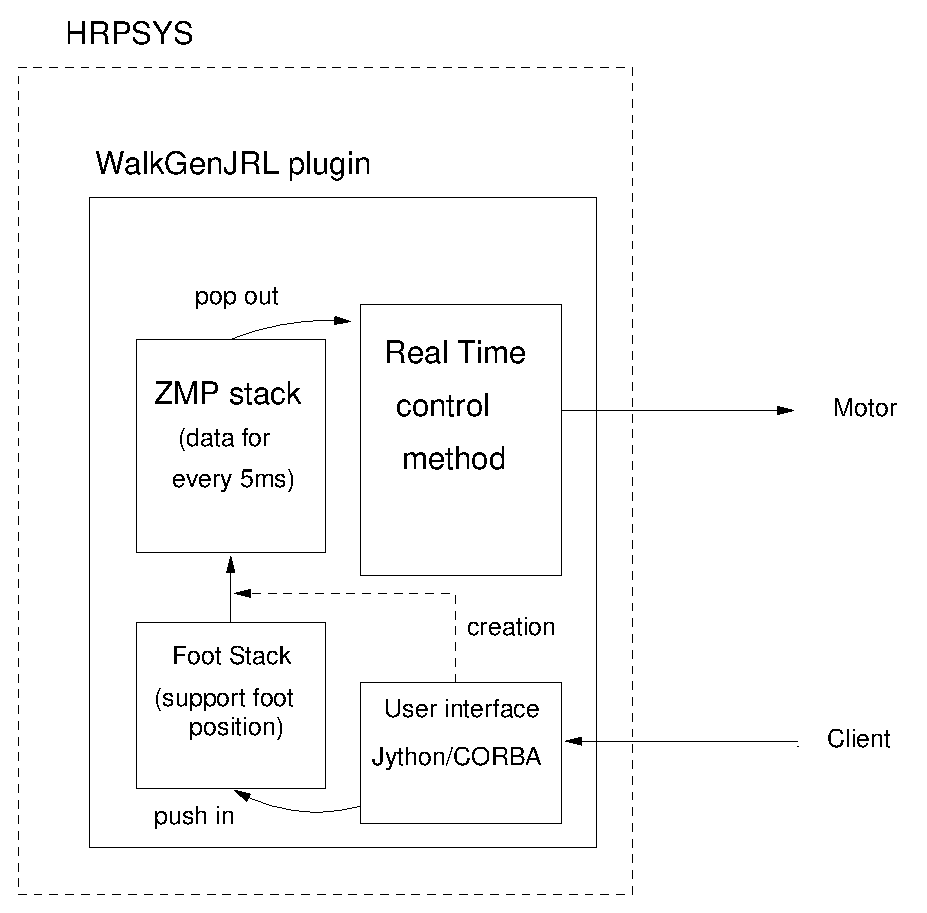
\includegraphics[width=0.7\linewidth]{./figures/PatternGenerator/Stacks}
\caption{Stacks organization and overview of the WalkGenJRL plugin's structure.}
\label{pic:Stacks}
\end{center}
\end{figure}

\subsection{Functionnalities}

This paragraph describes the functionnalities provided by WalkGenJRL.

\subsubsection{Foot positionning}

\begin{itemize}
\item {\bf stepseq}: Specify the ZMP trajectory by giving relative support foot positionning.
The ZMP is assumed to be under the CoM at the beginning of the motion.
A relative supporting foot position is given by three parameters $(dx_i,dy_i,\theta_i)$.
The parameter $\theta_i$ gives the angle by which the next foot orientation will be modified, and $(dx_i,dy_i)$ gives
the position of the next support foot position according to the direction.x
Fig \ref{pic:FootPositionning} gives an example of such a sequence.
At first the robot moves its support towards the left foot, switch to the right foot
20 cm ahead, then to the left foot with a rotation of 10 degrees, then to the right
foot with also a rotation of 10 degrees. You have to give the last motion for having 
the robot stop correctly. In this case, you should add the motion for bringing the left foot
at the same level than the right foot. Bringing the ZMP between the two foot is done 
automatically by the plugin. 

The final sequence is then:
\begin{verbatim}
:stepseq 0 0.095 0 0.2 0.19 0.0 0.2 -0.19 10.0 0.2 0.19 10.0 
0.0 -0.19 0.0 
\end{verbatim}
\begin{figure}[htb]
\begin{center}
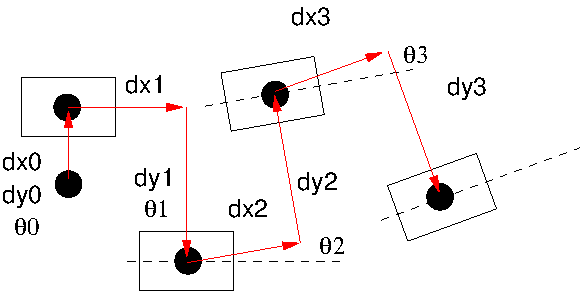
\includegraphics{./figures/PatternGenerator/FootPositionning}
\caption{Example of foot positionning: ( 0 0.095 0 , 0.2 0.19 0.0, 0.2 -0.19 10.0, 0.2 0.19 10.0) }
\label{pic:FootPositionning}
\end{center}
\end{figure}
The Jython interpreter will exit from this function before the motion
is completly finished. BUT the sequence will be performed as soon as
the function is exited.
Currently you have to wait the end of motion
by using a waitInputConfirm call.
It is unwise to add a new sequence while the motion is unfinished.

\begin{itemize}
\item \textbf{Jython availability:} yes
\item \textbf{Corba availability:} no
\item \textbf{Source code location:} Inside libWalkGenJRL.
\end{itemize}

\item {\bf arc}: The robot walks tangently to a specified arc.
This capability is supposed to be compatible with Kajita-San, however you might find 
some discrepencies. They are four parameters for this function : $(x,y,\theta,Foot)$,
where $(x,y)$ (in meters) is the center of the arc relative to the current position of the robot,
$\theta$ (degrees) the arc's angle, and $Foot$ the starting support foot ($-1$ : Right, $1$: Left).
The current strategy is the following:
\begin{equation}
\begin{aligned}
R &= \sqrt{x^2+y^2} \\
NbOfSteps &= \frac{\theta R }{StepMax} \\
NbOfStepsInt &= \lfloor NbOfSteps \rfloor \\
\theta_{steps} &= \frac{StepMax}{R} \\
\theta_{last} &= \theta - \theta_{steps} * NbOfStepsInt \\
\end{aligned}
\end{equation}
The robot perform $NbOfStepsInt$ of $\theta_{steps}$ degrees.
The last step is of $\theta_{last}$ degrees.
$StepMax$ is the maximum step length. It is fixed by default at 0.15 cm.
\par
The function will exit almost immediatly, and the motion will NOT
be performed unless you call the {\bf finish} function.
Before calling finish, it is strongly advice to use {\bf lastsupport}.

The internal algorithm puts footprint on each side of an arc.
Therefore the left foot trajectory and the right trajectory are on two arcs.
If we note $\Delta Feet$ the distance between the two feet along the $y-axis$ 
(in the OpenHRP frame), then the internal arc has a ray of $R - \Delta Feet$.
The external arc has a ray of $R + \Delta Feet$.
Considering the case depicted in figure \ref{pic:ArcAlgo2},
and assuming that $SF= -1$ if the support is the left foot,
and $SF=1$ if the support foot is the right foot, the coordinates
of the support foot is :	
\begin{equation*}
\begin{aligned}
x(k)_{sf} &= R + SF  \Delta Feet  sin(k \theta_{steps}) - (R-SF \Delta Feet ) sin(k \theta_{steps}) \\
y(k)_{sf} &= -(R + SF  \Delta Feet  cos(\theta_{steps}) - (R-SF \Delta Feet ) cos(k \theta_{steps}) )\\
\end{aligned}
\end{equation*}

In order to give the proper translation for the relative foot position
between support foot $k-1$ and $k$, we note $v_{w}$ this translation in the
world reference frame (as depicted in figure \ref{pic:ArcAlgo}). 
If $v_{i}$ is the same vector but expressed in the reference frame of support foot $k$,
then 
\begin{equation*}
v_w = {\bf R}_{k \theta_{steps}} v_i
\end{equation*}
One can remark that $v_i$ is the translation $(sx,sy)$ we are looking for.
Indeed the support foot $k$ has the proper orientation after $k \theta_{steps}$ rotation.
Then by computing $v_w = [ x(k)_{sf}-x(k-1)_{sf} \; y(k)_{sf}-y(k-1)_{sf} ]^T$, 
we get 
\begin{equation*}
v_i = {\bf R}^{-1}_{k \theta_{steps}} v_w = {\bf R}^{T}_{k \theta_{steps}} v_w
\end{equation*}


\begin{figure}[htb]
\begin{center}
\includegraphics[width=6cm]{./figures/PatternGenerator/arcalgo2}
\caption{Splitting the arc into small arc of $\theta_{steps}$ degrees}
\label{pic:ArcAlgo2}
\end{center}
\end{figure}
\begin{figure}[htb]
\begin{center}
\includegraphics[height=6cm]{./figures/PatternGenerator/arcalgo}
\caption{Computing $v_w$ into the reference frame of support foot $k$ }
\label{pic:ArcAlgo}
\end{center}
\end{figure}

\begin{itemize}
\item \textbf{Jython availability:} yes
\item \textbf{Corba availability:} no
\item \textbf{Source code location:} Inside WalkGenJRL plugin.
\end{itemize}

\item {\bf arccentered}: With this function the robot walks orthogonaly to 
an arc. They are four parameters for this function : $(x,y,\theta,Foot)$,
where $(x,y)$ (in meters) is the center of the arc relative to the current position of the robot,
$\theta$ (degrees) the arc's angle, and $Foot$ the starting support foot ($-1$ : Right, $1$: Left).
The current strategy is the following:
\begin{equation}
\begin{aligned}
R &= \sqrt{x^2+y^2} \\
NbOfSteps &= \frac{\theta R }{StepMax} \\
NbOfStepsInt &= \lfloor NbOfSteps \rfloor \\
\theta_{steps} &= \frac{StepMax}{R} \\
\theta_{last} &= \theta - \theta_{steps} * NbOfStepsInt \\
\end{aligned}
\end{equation}
The robot perform $NbOfStepsInt$ of $\theta_{steps}$ degrees.
The last step is of $\theta_{last}$ degrees.
\par
The function will exit almost immediatly, and the motion will NOT
be performed unless you call the {\bf finish} function.
Before calling finish, it is strongly advice to use {\bf lastsupport}.

\begin{itemize}
\item \textbf{Jython availability:} yes
\item \textbf{Corba availability:} no
\item \textbf{Source code location:} Inside WalkGenJRL plugin.
\end{itemize}

\item {\bf lastsupport}: This function generates a finishing sequence in the foot stack in order to make sure
 that the robot will perform a half-sitting position.
\par
The function will exit almost immediatly, and the motion will NOT
be performed unless you call the {\bf finish} function.

\begin{itemize}
\item \textbf{Jython availability:} yes
\item \textbf{Corba availability:} no
\item \textbf{Source code location:} Inside WalkGenJRL plugin.
\end{itemize}

\item {\bf finish}: This function will send the complete foot stack into 
the ZMP stack to be run by control loop.
The function will return only after the completion of the motion.

\begin{itemize}
\item \textbf{Jython availability:} yes
\item \textbf{Corba availability:} no
\item \textbf{Source code location:} Inside WalkGenJRL plugin.
\end{itemize}

\end{itemize}

\subsubsection{Walking parameters}
\begin{itemize}
\item {\bf omega}: Modify the angle for the foot landing and taking-off. This feature was intended to modify
the angle with which the robot land or take-off the support foot. It is currently set by default to 0.
It has never been tried yet into the real robot.
\begin{itemize}
\item \textbf{Jython availability:} yes
\item \textbf{Corba availability:} no
\item \textbf{Source code location:} Inside ZMPDiscretization.cpp (libWalkGenJRL).
\end{itemize}


\item {\bf stepheight}: Modify the height with which the robot will perform a step.  
It is currently set by default to 0.12 m. Has been tested on the real robot.
The unit is in meters.
\begin{itemize}
\item \textbf{Jython availability:} yes
\item \textbf{Corba availability:} no
\item \textbf{Source code location:} Inside ZMPDiscretization.cpp (libWalkGenJRL).
\end{itemize}

\item {\bf singlesupporttime}: Modify the duration of the single support time. 
The current rule is to have 
\begin{equation}
singlesupporttime+doublesupporttime=0.8 s
\end{equation}
Has been tested on the real robot. The default value is 0.78
The unit is in seconds.
\begin{itemize}
\item \textbf{Jython availability:} yes
\item \textbf{Corba availability:} no
\item \textbf{Source code location:} Inside ZMPDiscretization.cpp (libWalkGenJRL).
\end{itemize}

\item {\bf doublesupporttime}: Modify the duration of the double support time. 
The current rule is to have 
\begin{equation}
singlesupporttime+doublesupporttime=0.8 s
\end{equation}
Has been tested on the real robot.
 The default value is 0.02. The unit is in seconds.
\begin{itemize}
\item \textbf{Jython availability:} yes
\item \textbf{Corba availability:} no
\item \textbf{Source code location:} Inside ZMPDiscretization.cpp (libWalkGenJRL).
\end{itemize}

\end{itemize}

\chapter{The theory behind}

\section{Inverse Kinematics}
\subsection{The legs}
The main purpose of this paragraph is to compute the joint values
for a given position and orientation of an hip joint (RLEG\_JOINT0
or LLEG\_JOINT0) and the corresponding foot. 
From the specification of the HRP-2 robot, the right leg of the robot
can be represented by a sticky drawing depicted in figure \ref{pic:InverseKinematicsforHRP2}.
They are some slight differences compare to the part described in Kajita \cite{Kajita2005}.
%
\begin{figure}[htb]
\begin{center}
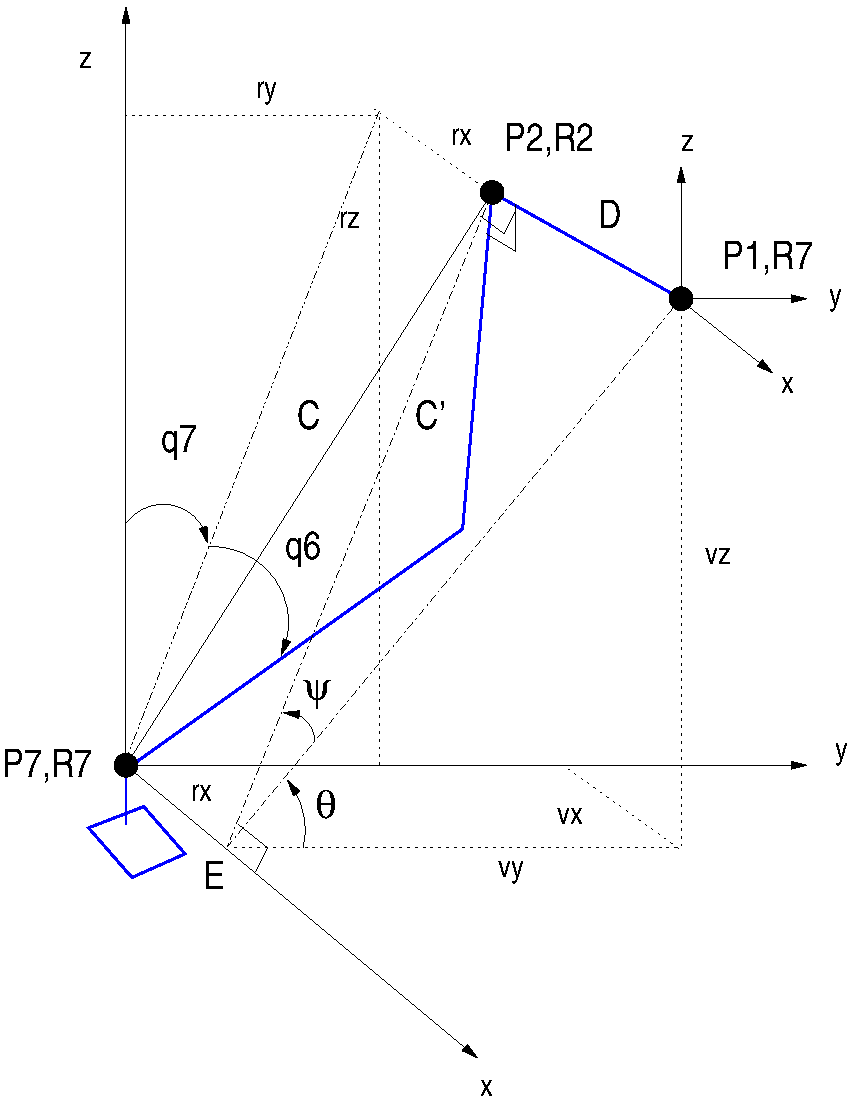
\includegraphics[width=0.5\linewidth]{./figures/PatternGenerator/InverseKinematics2}
\caption{Inverse Kinematics for the HRP-2 robot}
\label{pic:InverseKinematicsforHRP2}
\end{center}
\end{figure}
%
Indeed in this case, the leg of the robot can be seen as rotating around the ankle of the foot,
until it is tangent to a sphere $D$ around the hip position.
Therefore the segment  $(P2,P1)$ is orthogonal to the leg plane.
If $P1$ is expressed in the reference frame of $P7$, it is then 
quite simple to find $C'$, $\theta$ and $\Psi$.
Indeed, assuming that $P1= { v_x, v_y, v_z}$ and $P2 = {r_x, r_y, r_z}$ then : 
\begin{equation}
\begin{aligned}
r_x &= v_x \\
C' &= \sqrt{v_x^2 + v_z^2 - D^2} \\
\psi &= atan(D,C') \\
\theta &= atan(v_z, v_y) \\
r_y &= cos(\psi+\theta) *C_p \\
r_z &= sin(\psi+\theta) *C_p \\
\end{aligned}
\end{equation}
where $C'$ is the distance between $P_2$ and the point $E$. $E$ is intersecting $P_7$'s $x$-axis and 
the plan orthogonal to this axis, which includes $P_2$ and $P_7$.
$\psi$ is the angle between $(E, P_1)$ and $(E,P_2))$.
$\theta$ is the angle between $(E,P_1)$ and the $(x,y)$-plane.

Once all the values ${ r_x, r_y, r_z}$ are known 
it is possible to reuse the same arguments than in \cite{Kajita2003}.
Indeed:
\begin{equation*}
C = \sqrt{r_x^2 + r_y^2 + r_z^2}
\end{equation*}
It is then possible to compute $q_5$ as:
\begin{equation*}
q_5 = -cos^{-1}( \frac{A^2 + B^2 - C^2}{2AB}) + \pi
\end{equation*}

\begin{equation*}
\frac{C}{sin(\pi - q_5)}= \frac{A}{sin \alpha}
\end{equation*}
\begin{equation*}
\alpha = asin( \frac{A sin(\pi - q_5)}{C})
\end{equation*}

\begin{equation*}
\begin{aligned}
q_5 &= atan2(r_y,r_z)\\
q_6 &= -atan2(r_x,sign(r_z)\sqrt{r_x^2 + r_y^2} - \alpha\\
\end{aligned}
\end{equation*}


\begin{equation*}
{\bf R}_7 = {\bf R}_1 {\bf R}_z(q_2){\bf R}_x(q_3){\bf R}_y(q_4) {\bf R}_y(q_5+q_6) {\bf R}_x(q_7)
\end{equation*}

\begin{equation*}
{\bf R}_z(q_2) {\bf R}_x(q_3) {\bf R}_y(q_4) = {\bf R}^T_1 {\bf R}_7 {\bf R}_x(q_7) {\bf R}_y (q_5 +q_6)
\end{equation*}

Then:

\begin{equation*}
\left[
\begin{matrix}
c_2 c_4-s_2 s_3 s_4   & -s_2 c_3 & c_2 s_4 + s_2 s_3 c_4 \\
s_2 c_4 + c_2 s_3 s_4 &  c_2 c_3 & s_2 s_4 - c_2 s_3 c_4 \\
-c_3 s_4 & s_3 & c_3 c4\\
\end{matrix}
\right]
=
\left[
\begin{matrix}
R_{11} & R_{12} & R_{13} \\
R_{21} & R_{22} & R_{23} \\
R_{31} & R_{32} & R_{33} \\
\end{matrix}
\right]
\end{equation*}

\section{Dynamic models of biped robot}

\subsection{3D Linear Inverted Pendulum Mode and Zero-moment point}

``In this context a constraint control is applied to an inverted pendulum,
such that the mass should move along an arbitrary predefined plane.
The subsequent model is called the \textit{Three-Dimensional Linear Inverted Pendulum Model} (3D-LIPM). 
We take Cartesian coordinates as shown
in figure \ref{pic:PendulumUnderConstraint} and specifiy the $x$-axis as the ordinal walking 
direction. The constraint plane is represented with given normal
vector ($k_x,k_y,-1$) and $z$ intersection $z_c$ as:
\begin{equation}
z = k_x x + k_y y + z_c
\label{eq:ConstraintPlane}
\end{equation}
\begin{figure}[htb]
\begin{center}
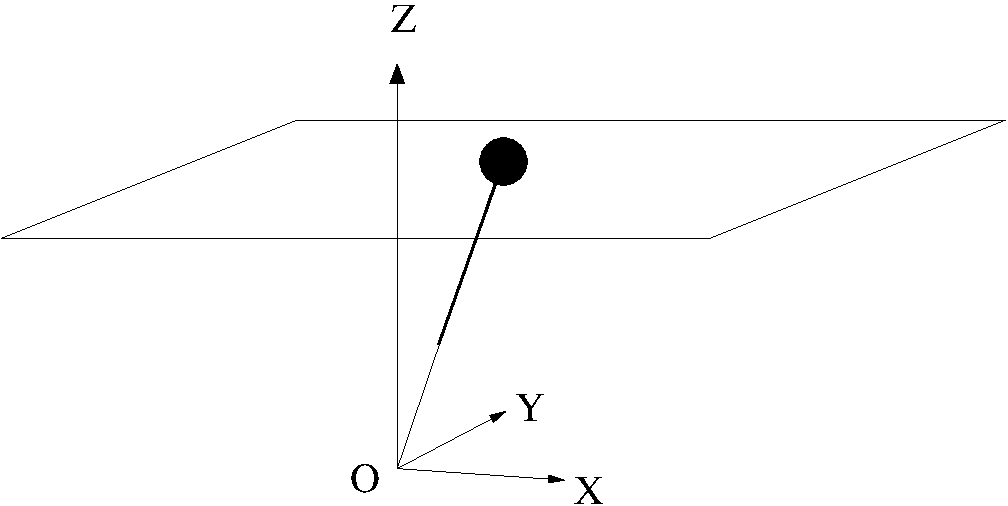
\includegraphics[width=0.5\linewidth]{./figures/PatternGenerator/PendulumUnderConstraint}
\caption{Pendulum under constraint}
\label{pic:PendulumUnderConstraint}
\end{center}
\end{figure}

If the constraint plane is horizontal ( $k_x = k_y = 0$),
the dynamics under the constraint control is given by
\begin{equation}
\ddot{y} = \frac{g}{z_c} y - \frac{1}{m z_c} \tau_x 
\label{eq:DynConstraintLawY}
\end{equation}

\begin{equation}
\ddot{x} = \frac{g}{z_c} x - \frac{1}{m z_c} \tau_y 
\label{eq:DynConstraintLawX}
\end{equation}

where $m$ is the mass of the pendulum, $g$ is the gravity acceleration
and $\tau_x, \tau_y$ are the torques around $x$-axis and $y$-axis
respectively. This pendulum under constraint is depicted in figure \ref{pic:PendulumUnderConstraint}.
\par
Even in the case of the sloped constraint where $k_x$,$k_y \neq 0 $, 
we can obtain the same dynamics by applying additional constraint
\begin{equation}
\tau_x x + \tau_y y  = 0
\label{eq:ConstraintTorque}
\end{equation}
for the input torques.

Equations \ref{eq:DynConstraintLawY} and \ref{eq:DynConstraintLawX} are linear
equations. The only parameter which govens those dynamics is $z_c$, i.e., the
$z$ intersection of the constraint plane and the inclination of the plane never
affects the horizontal motion.
\par
For the 3D-LIPM with the horizontal constraint ($k_x = k_y = 0$), we can easily
calculate the zero-moment point (ZMP), which is widely used in biped robot
research \cite{}.
\begin{equation}
p_x = -\frac{\tau_y}{m g }\\
p_y = \frac{\tau_x}{m g }\\
\label{eq:ZMP}
\end{equation}
where $(p_x,p_y)$ is the location of the ZMP on the floor.
By substituing equations \ref{eq:ZMP} to the 3D-LIPM (\ref{eq:DynConstraintLawY}
and \ref{eq:DynConstraintLawX}) we obtain:
\begin{equation}
\ddot{y} = \frac{g}{z_c}(y-p_y) \\
\label{eq:DynZMPY}
\end{equation}
\begin{equation}
\ddot{x} = \frac{g}{z_c}(x-p_x) \\
\label{eq:DynZMPX}
\end{equation}
\begin{figure}[htb]
\begin{center}
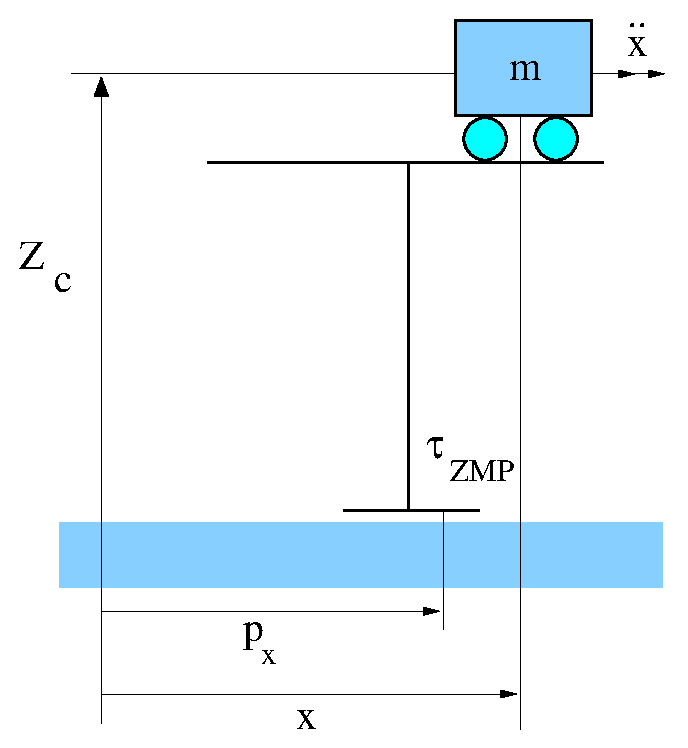
\includegraphics[width=0.5\linewidth]{./figures/PatternGenerator/CartTableModel}
\caption{The Cart table model}
\label{pic:CartTableModel}
\end{center}
\end{figure}

\subsection{ZMP equations and cart-table model}
To control the ZMP, it should appears in the outputs of the system formula.
However in 3D-LIPM as described in the last section, it appears to 
be the input of the system. Therefore equations \ref{eq:DynZMPY} and \ref{eq:DynZMPX}
are rewritten to have the ZMP with the following form:
\begin{equation}
p_y = y - \frac{z_c}{g} \ddot{y} 
\label{eq:ZMPY}
\end{equation}
\begin{equation}
p_x = x - \frac{z_c}{g} \ddot{x} 
\label{eq:ZMPX}
\end{equation}
In the remainder of this chapter, we will refer to the above equations as the \textit{ZMP equations}.
\par
Figure \ref{pic:CartTableModel} shows a suggestive model directly corresponds to these equations.
It depicts a running cart of mass $m$ on a pedestal  table whose mass
is negligible (we need two sets of a cart on a table for the motion $x$ and $y$).
\par
As shown in the figure, the foot of the table is too small to let the cart stay on the edge.
However if the cart accelerates with a proper rate, the table can keep upright for
a while. At this moment, the ZMP exists inside of the table's foot.
Since the moment around the ZMP must be zero, we have:
\begin{equation}
\tau_{zmp} = mg(x-p_x) - m \ddot{x} z_c = 0
\end{equation}
We can verify that this yields to the equation \ref{eq:ZMPX}.

\section{Walking pattern generation for a given ZMP}
%
\begin{figure}[htb]
\begin{center}
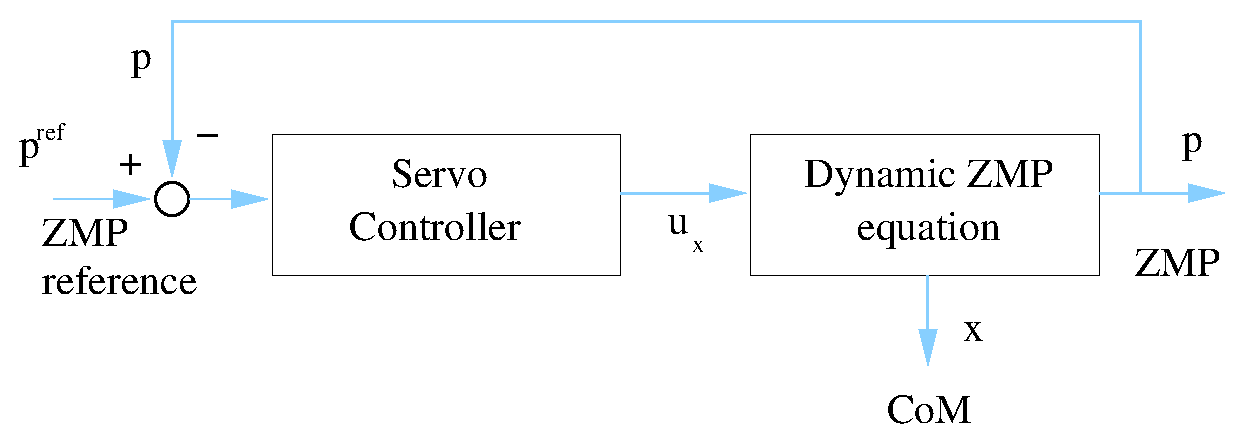
\includegraphics[width=0.5\linewidth]{./figures/PatternGenerator/PatternGenerationAsZMPTrackingControl}
\caption{Pattern Generation as ZMP tracking control}
\label{pic:PatternGenerationAsZMPTrackingControl}
\end{center}
\end{figure}
%
\subsection{Pattern generation as an inverse problem}

When we represent a robot as the cart-table model and give
the cart motion as the trajectory of the center of mass (CoM) of the robot,
we can easily calculate the resulted ZMP by using the ZMP equations
\ref{eq:ZMPY} and \ref{eq:ZMPX}.
On the other hand, a walking pattern generation is the inverse problem of
this. That is, the cart motion should be calculated from the given ZMP
trajectory which is determined by the desired footholds and step period.
\par
Takanishi et al. proposed to solve this problem by using Fourier Transformation.
By applying the Fast Fourier Transformation (FFT) to the ZMP reference,
the ZMP equations can be solved in frequency domain. Then the inverse
FFT returns the resulted CoM trajectory into time domain.
\par
Kagami, Nishiwaki et al. proposed a method to solve this problem in the discrete
time domain. They showed that the ZMP equation can be discretized as a trinomial expression,
and it can be efficiently solved by an algorithm of $O(N)$ for the given reference data
of size $N$.
\subsection{ZMP control as a servo problem}
Let us define a new variable $u_x$ as the time derivate of the horizontal acceleration of CoM.
\begin{equation}
\frac{d}{dt}\ddot{x} = u_x
\label{eq:CoMAcceleration}
\end{equation}

Regarding $u_x$ as the input of equation \ref{eq:ZMPX}, it is possible to translate the ZMP
equation into a strictly proper dynamical system as:
\begin{equation}
\begin{aligned}
\frac{d}{dt}
\left[ 
\begin{matrix}
x \\
\dot{x} \\
\ddot{x} \\
\end{matrix}
\right] &=
\left[
\begin{matrix}
0 & 1 & 0 \\
0 & 0 & 1 \\
0 & 0 & 0 \\
\end{matrix}
\right]
\left[ 
\begin{matrix}
x \\
\dot{x} \\
\ddot{x} \\
\end{matrix}
\right]
+
\left[ 
\begin{matrix}
0 \\
0 \\
1 \\
\end{matrix}
\right]
u_x \\
p_x &= [ 1 \; 0 \; -\frac{z_c}{g} ] 
\left[ 
\begin{matrix}
x \\
\dot{x} \\
\ddot{x} \\
\end{matrix}
\right]
\end{aligned}
\label{eq:DynamicalSystem}
\end{equation}
%
\begin{figure}[htb]
\begin{center}
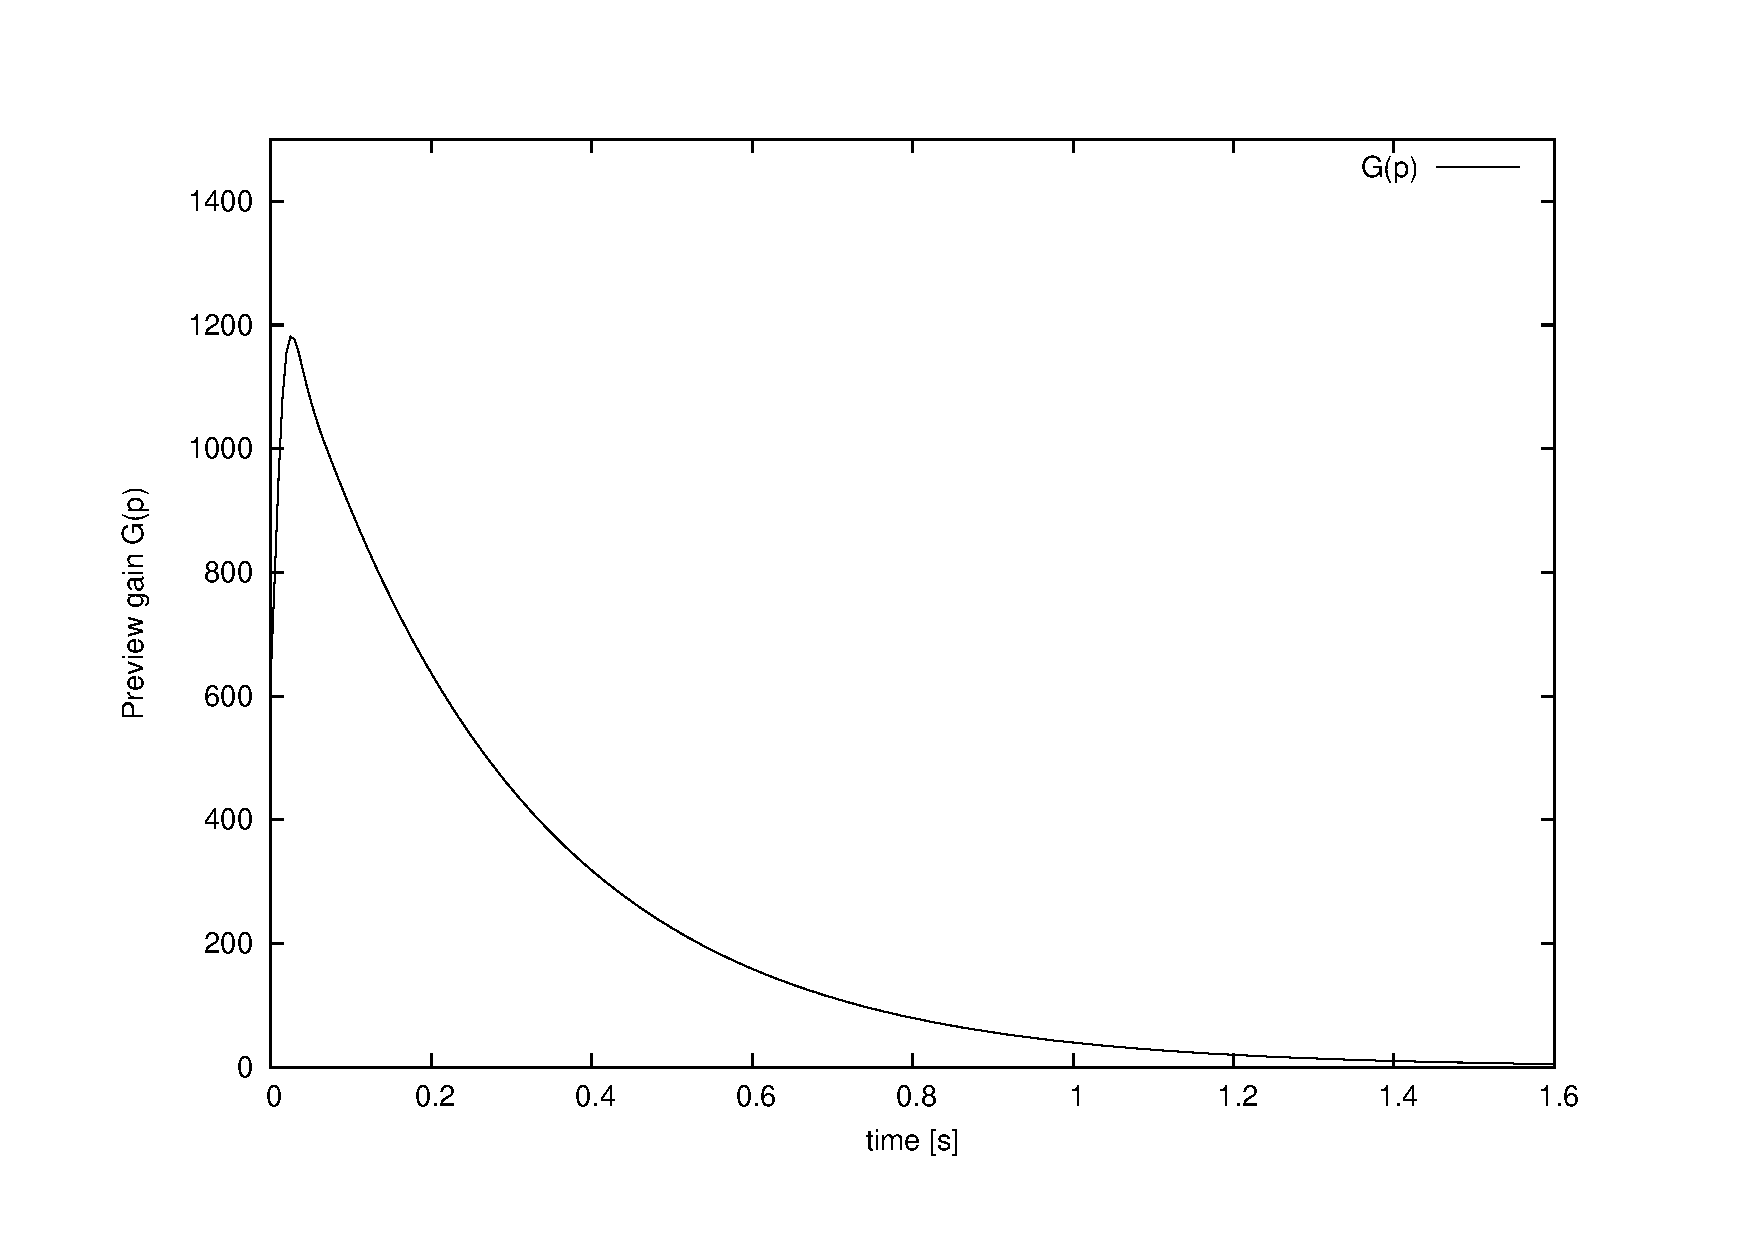
\includegraphics[width=0.5\linewidth]{./figures/PatternGenerator/PreviewGains}
\caption{Preview controller gain $G_p$ ($T = 5$[ms], $z_c=0.814$ [m])}
\label{pic:PreviewGains}
\end{center}
\end{figure}
%
For equation \ref{eq:ZMPY}, $u_y$ is defined in the same manner, and a similar system is found.
\par
By using the dynamics of equation \ref{eq:DynamicalSystem} we can construct a walking pattern 
generator as a ZMP tracking control system. The system generates the CoM trajectory such 
that the resulted ZMP follows the given reference.
However, we must consider an interesting feature of this problem as follows.
Figure 
%\ref{}
illustrates the ideal trajectories of the ZMP and the CoM of a robot that walks one step forward
dynamically. The robot supports its body by hind-leg from 0s to 1.5s, and has a support 
exchange at 1.5s followed by the foreleg support until 3.0s. Thus the reference ZMP should have
a step change at 1.5s and obviously the CoM must start moving \textit{before} this.
Assuming the controller in Figure \ref{pic:PatternGenerationAsZMPTrackingControl} , the output must be calculated from the future input !
\par
Although this sounds curious, we do not have to violate the law of causality.
Indeed we are familiar with such situation in driving on a winding road, where we steer
a car by watching ahead, that is, watching the future reference.
\par
A control that utilizes future information was first proposed by Sheridan in 1966 and was named
``Preview control'' . In 1969, Hayase and Ichikawa worked on the same concept and solved 
a linear quadratic (LQ) optimal servo controller with preview 
action. A digital version of LQ optimal preview controller was developed
by Tomizuka and Rosenthal in 1979 and was completed as the controller
for MIMO system by Katayama et al. in 1985.
%
\clearpage
\begin{figure}[htb]
\begin{center}
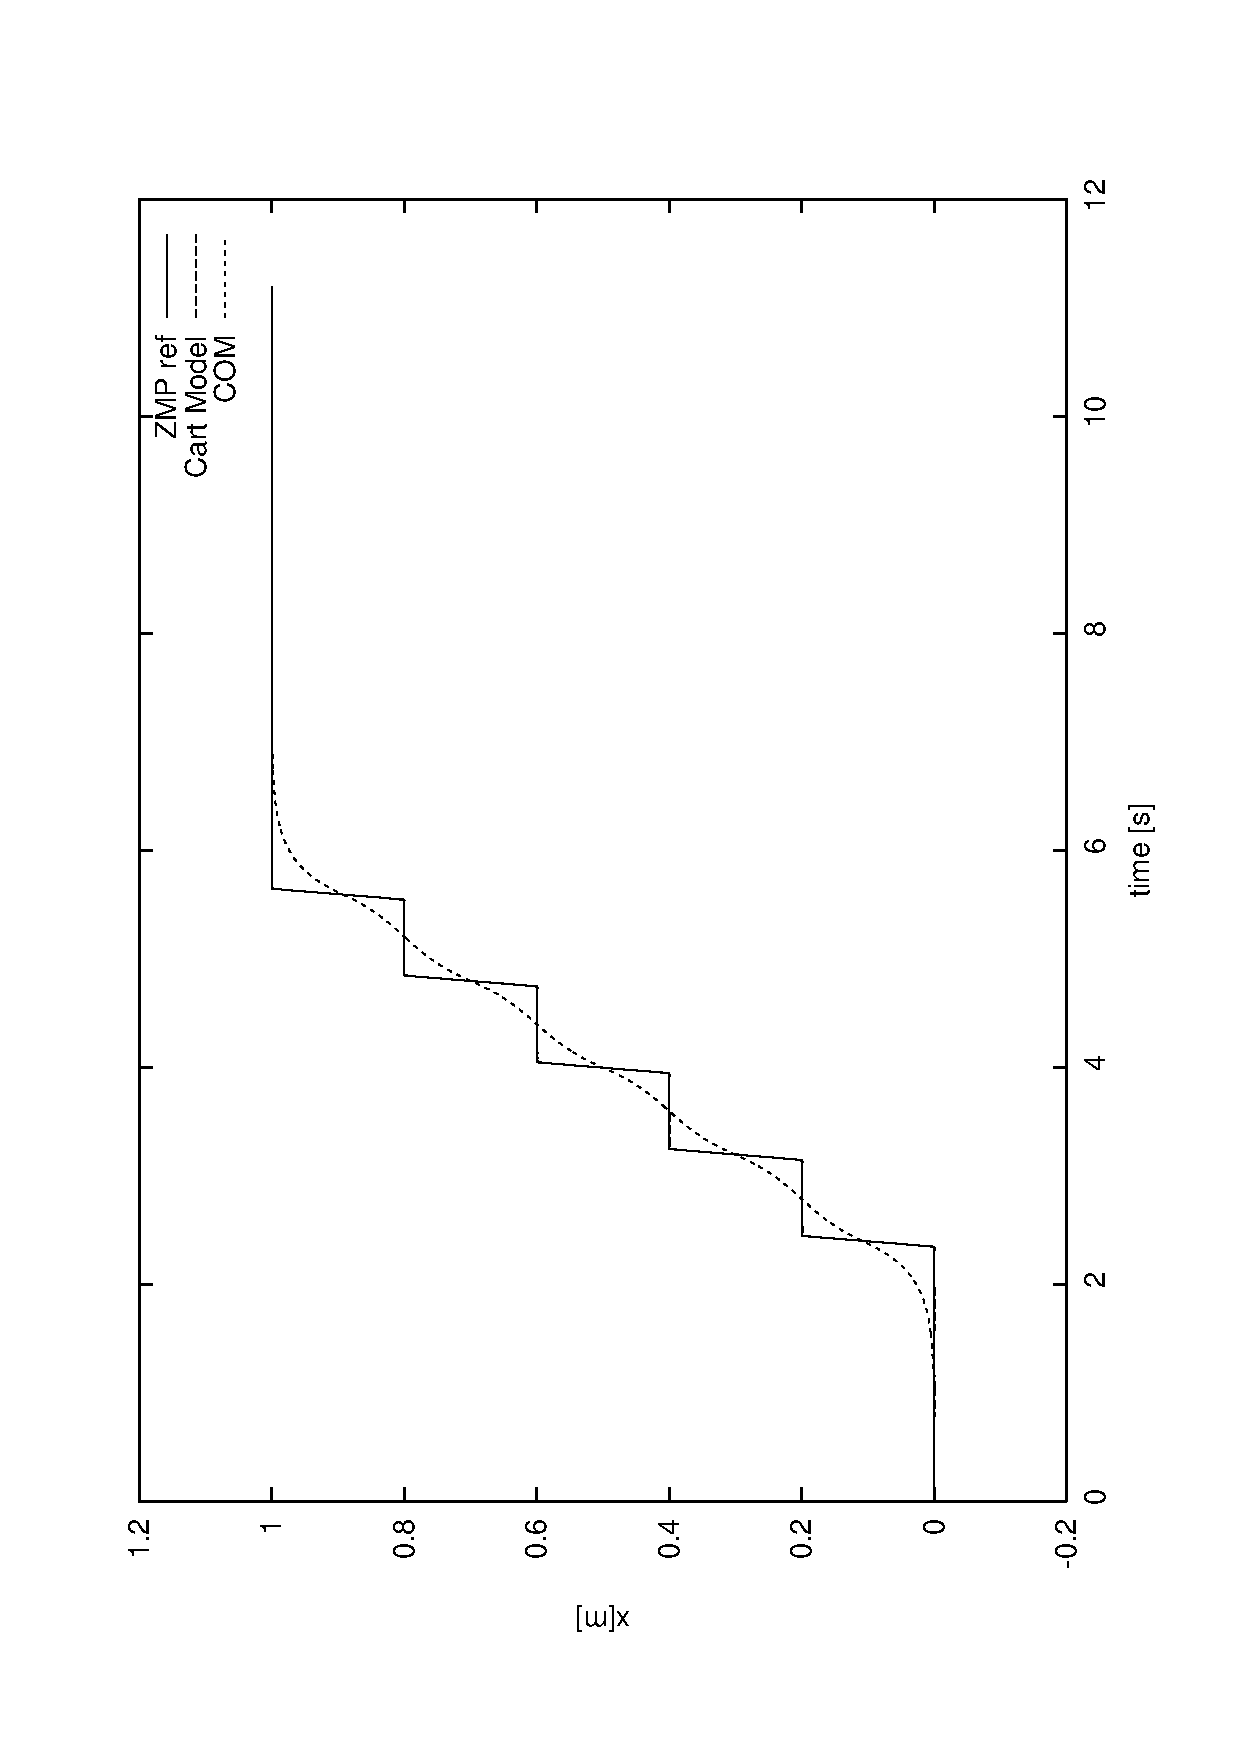
\includegraphics[width=\linewidth]{./figures/PatternGenerator/FigurePC1_X}
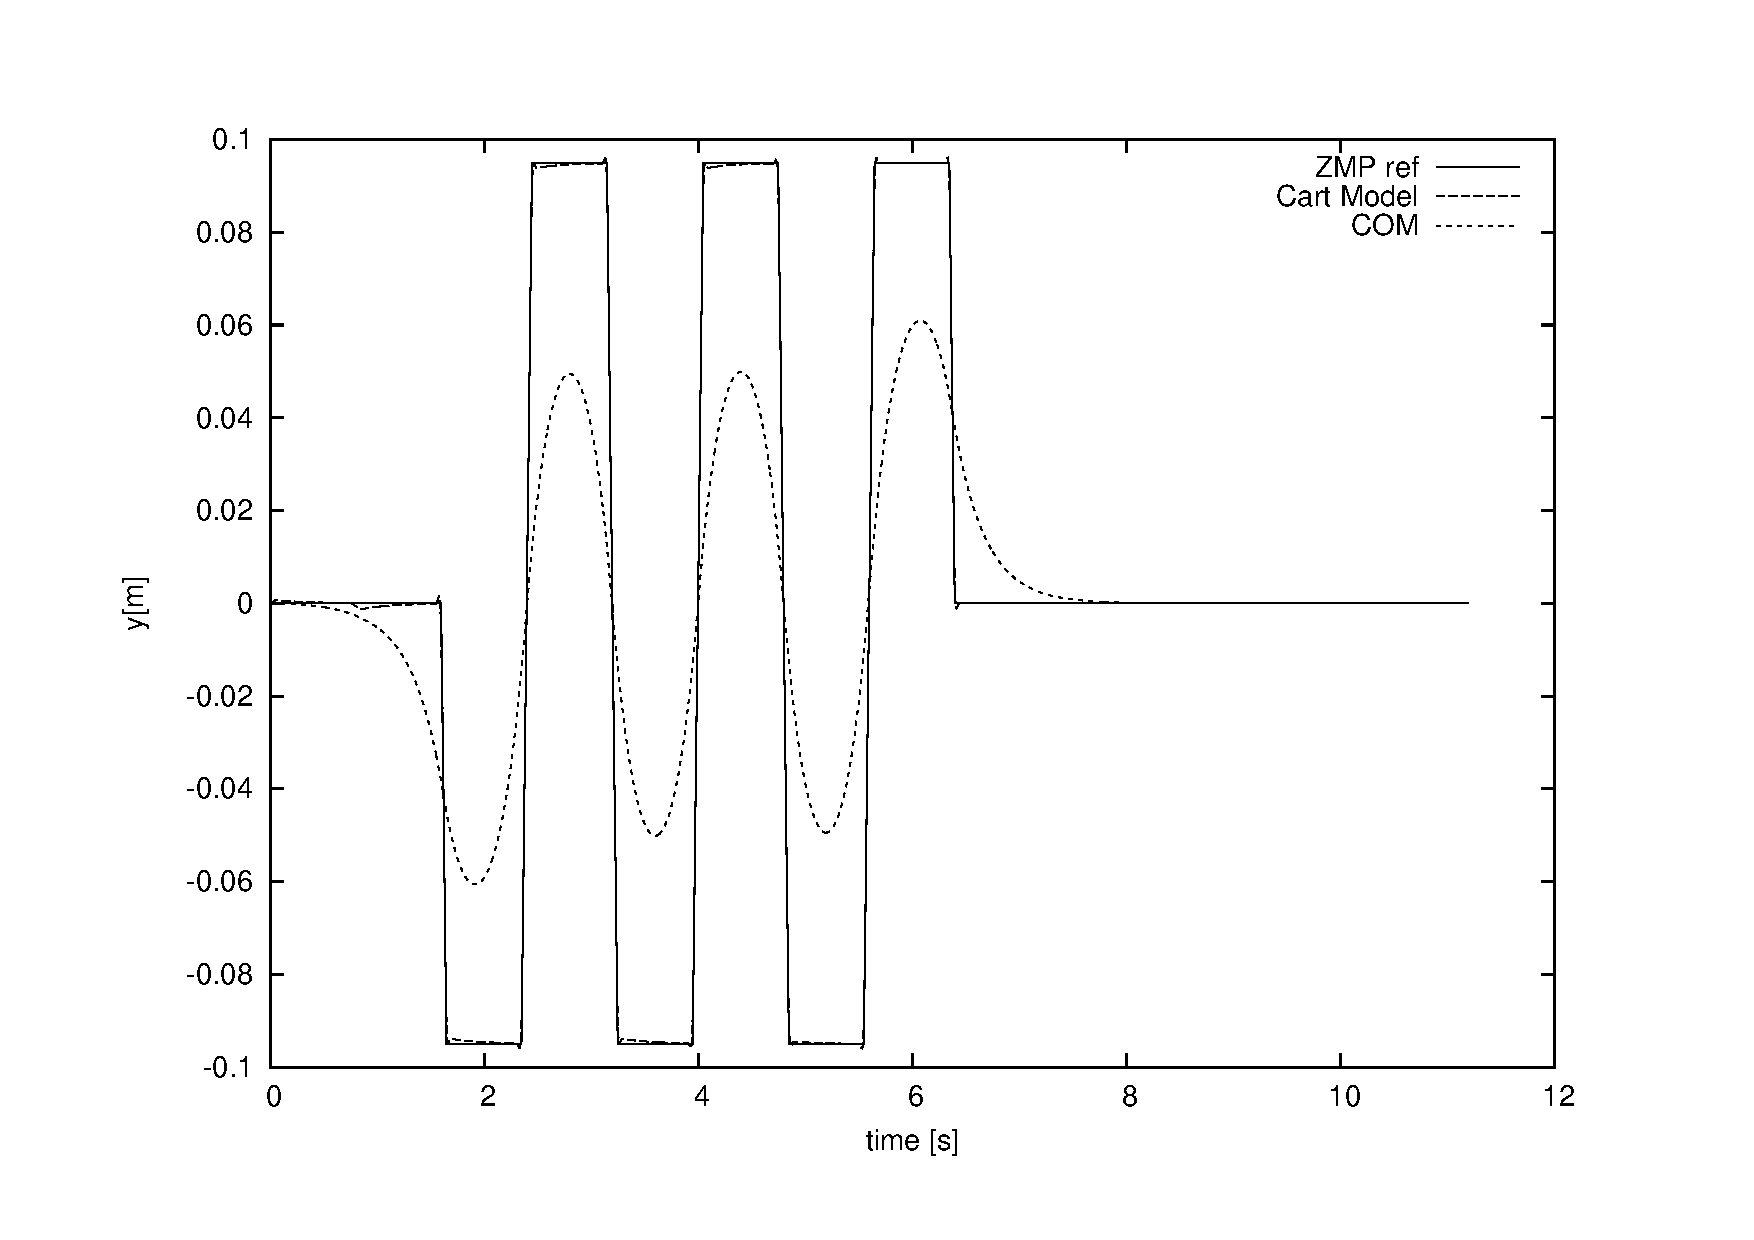
\includegraphics[width=\linewidth]{./figures/PatternGenerator/FigurePC1_Y}
\caption{Body trajectory obtained by preview control, previewing period $T * NL = 1.6$ }
\label{pic:BodyTrajectory}
\end{center}
\end{figure}
\clearpage
\subsection{Pattern generation by preview control}
Let us design an optimal preview servo controller following the method proposed
by Katayama et al. 
\par
First, we discretize the system of equation \ref{eq:DynamicalSystem} with sampling
 time of $T$ as:
\begin{equation}
\begin{aligned}
{\bf x}(k+1) &= {\bf Ax} (k) + {\bf B}u(k),\\
p(k) &= {\bf Cx}(k),
\end{aligned}
\label{eq:DiscreteDS}
\end{equation}
where
\begin{equation}
\begin{aligned}
\bf{x}(k) & \equiv [ {\bf x}(k)\; \dot{\bf x}(k)\; \ddot{\bf x}(kT) ]^T , \\
u(k) & \equiv {\bf u}_x(kT) , \\
p(k) & \equiv {\bf p}_x(kT) , \\
{\bf A} & \equiv 
\left[
\begin{matrix}
1 & T & T^2/2 \\
0 & 1 & T \\
0 & 0 & 1
\end{matrix}
\right],\\
{\bf B} & \equiv 
\left[
\begin{matrix}
T^3/6 \\
T^2/2 \\
T
\end{matrix}
\right],
&
{\bf C}  \equiv
\left[
1 \; 0 \; \frac{-z_c}{g}
\right]
\end{aligned}
\end{equation}
\clearpage
\begin{figure}[htb]
\begin{center}
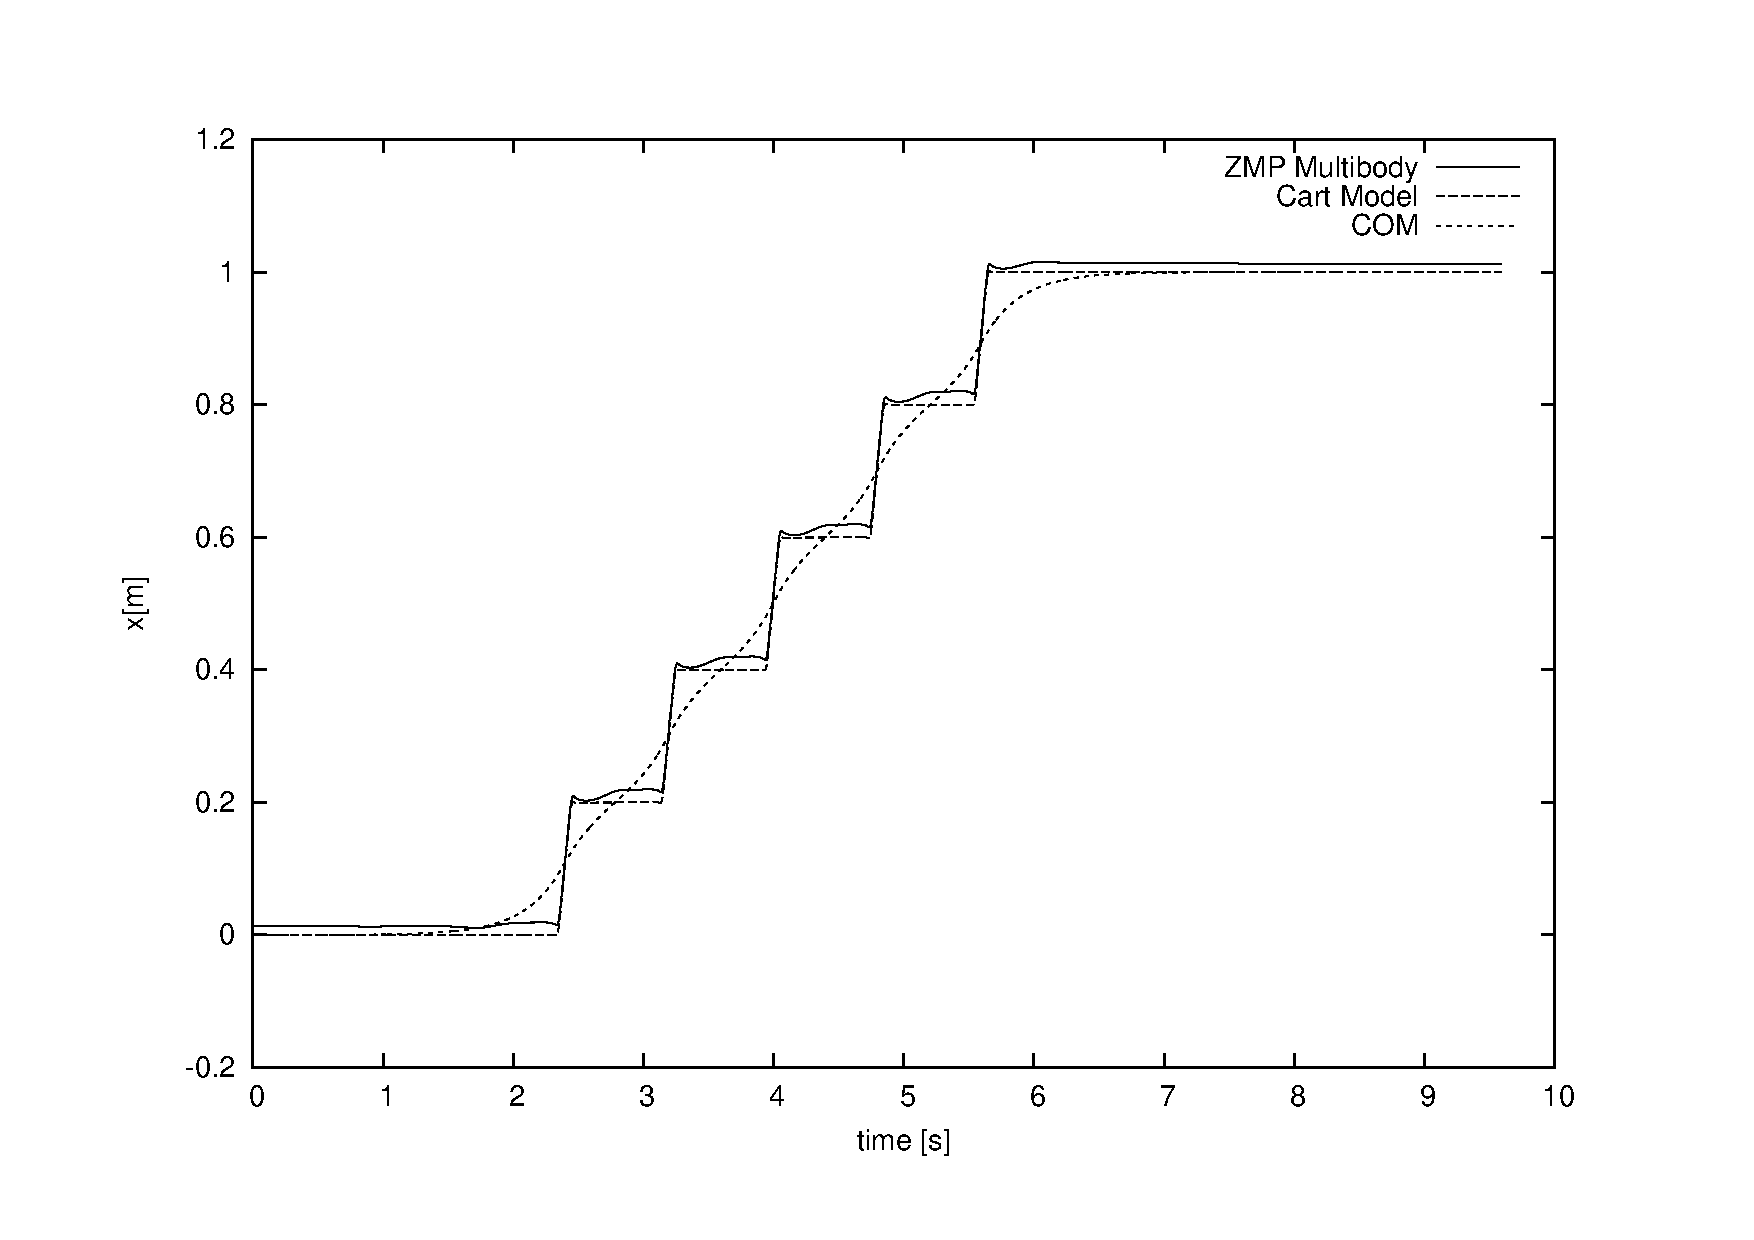
\includegraphics[width=\linewidth]{./figures/PatternGenerator/SecondFigureZMPMB_X}
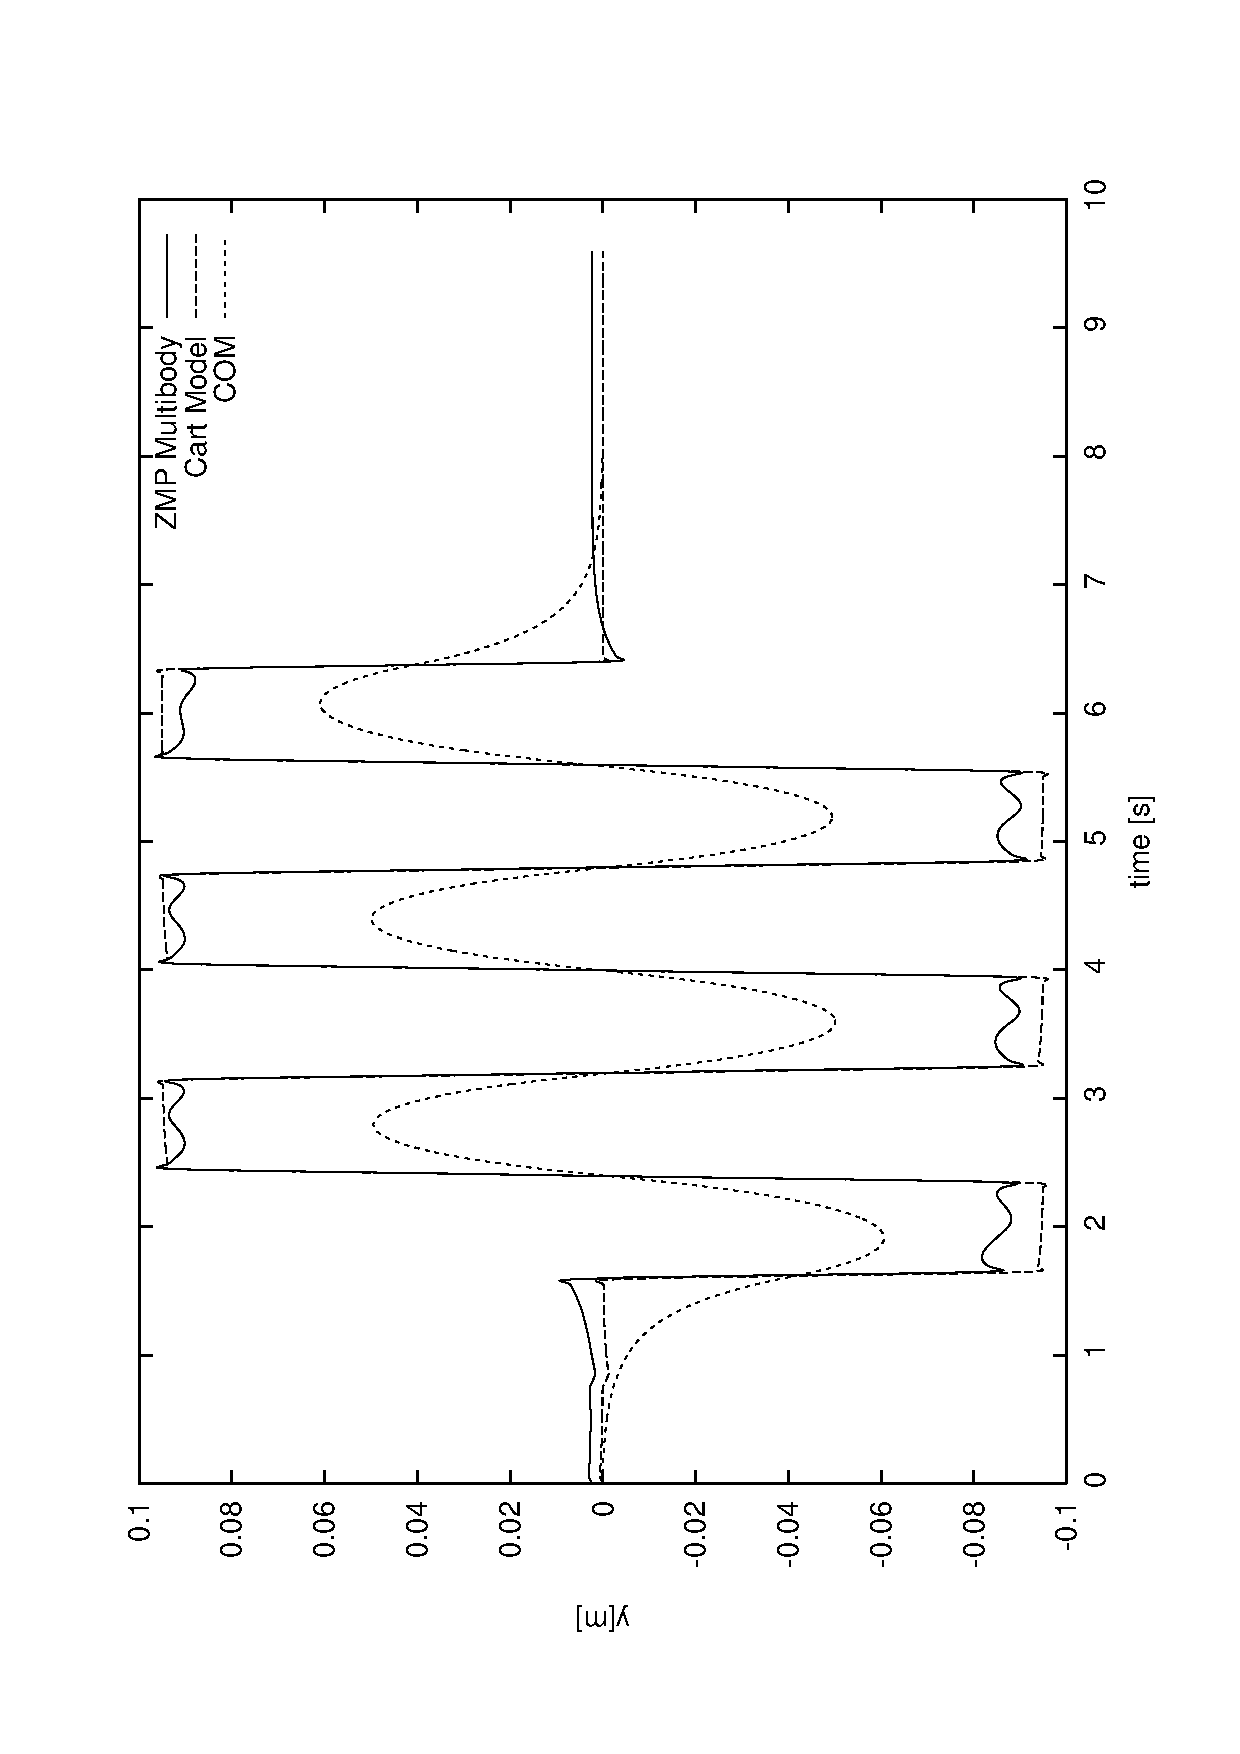
\includegraphics[width=\linewidth]{./figures/PatternGenerator/SecondFigureZMPMB_Y}
\caption{Body trajectory obtained by preview control, previewing period $T * NL = 1.6$ }
\label{pic:ZMPMB}
\end{center}
\end{figure}
\clearpage
With the given reference of ZMP $p^{ref}(k)$, the performance
index is specified as:
\begin{equation}
J = \sum^{\infty}_{i=k} \{ Q_ee(i)^2 + \Delta{\bf x}^T {\bf Q}_x \Delta{\bf x}(i) +
R \Delta u^2(i) \}
\label{eq:PerformanceIndex1}
\end{equation}
where $e(i) \equiv p(i) - p^{ref}(i)$ is the servo error, $Q_e,R > 0$ and ${\bf Q}_x$ is 
a $3 \times 3$ symmetric non-negative definite matrix.
$\Delta {\bf x} (k) \equiv {\bf x}(k) {\bf x}(k-1)$ is the incremental state vector
and $\Delta u(k) \equiv u(k) - u(k-1)$ is the incremental input.
\par
When the ZMP reference can be previewed for $N_L$ step future at every sampling time,
the optimal controller which minimizes the performance index \ref{eq:PerformanceIndex1}
is given by:
\begin{equation}
u(k) = -G_1 \sum^k_{i=0} e(i) - G_2{\bf x}(k) - \sum^{N_L}_{j=1}G_p(j) p^{ref}(k+j)
\end{equation}
where $G_1, G_2$ and $G_p(j)$ are the gains calculated from the weights $Q_e, {\bf Q}_x, R$
and the system parameter of \ref{eq:DiscreteDS}.
\par 
The preview control is made of three terms, the integral action on the tracking error,
the state feedback and the preview action using the future reference.
\par
Figure \ref{pic:PreviewGains} shows the gain for the preview action. We see the controller does not need
the information of far future because the magnitude of the preview gain $G_p$ becomes
very small in the future farther than 2 seconds.
\par
Figure \ref{pic:BodyTrajectory} is an example of walking pattern generation with the previewing period of 1.6s.
The upper graph is the sagittal motion along the $x$-axis and the lower graph is the
lateral motion along the $y$-axis. We can see a smooth trajectory of CoM (dashed line)
is generated and the resulted ZMP (bold line) follows the reference (thin line) with good
accuracy. The generated walking pattern corresponds to the walking of three steps forward.
The ZMP reference is designed to stay in the center of support foot during single
support phase, and to move from an old support foot to a new support foot during double
support phase. 
To obtain a smooth ZMP trajectory in double support, we filtered the generated ZMP
by an Infinite Impulse Response filter.
\par
Figure 8 is the result with the previewing period of 0.8s, which is not sufficient for the
ZMP tracking. In this case, the resulted ZMP (bold line) does not follow the reference
(thin line) well. We observe undershooting in the sagittal motion and overshooting in the 
lateral motion. It should be noted that even ZMP tracking performance is poor, the 
system still remains stable thanks to term of the state feedback.
\subsection{Pattern generation for multibody model}
The walking pattern is calculated by solving an inverse kinematics such that the CoM
of the robot follows the output of the preview controller. As the simpler implementation, we can 
also use the center of the pelvis link since it approximates the motion of the CoM.
\par
If the ZMP error becomes too big relative to the stability margin determined by the foot geometry,
the robot can fall. To fix the ZMP error, again we can use the preview control. That
is, we first calculate the CoM trajectory from the table-cart model and
obtain an expected ZMP error from the multibody model.
These information are stored to the buffer memory and loaded to be used after a delay time
of $T*N_L$. This way, we can use the \textit{future ZMP error} for the preview control 
to calculate a proper compensation.
Indeed by substraction a $\Delta_{ZMP}$ is computed and put inside a preview controller.
Because the discrete dynamic system is linear the variation of the CoM can be directly 
added to the cart-model CoM.
\par
Figure \ref{pic:ZMPMBcompensated}, shows the improved pattern of ZMP by this method. We can observe now the ZMP
computed by the multibody model (bold line) follows well the reference ZMP of the cart-table
model (thin line). The maximum ZMP error was 1.2 cm in the $x$-direction and $0.4 cm$ in $y$-direction.
We used the previewing period  $T*N_L$ = 1.6 (s) for this calculation. 
In \cite{Kajita2003} a shorter period was used and it happend to be effective enough 
because the amount of the compensation is small.
%
\clearpage
\begin{figure}[h]
\begin{center}
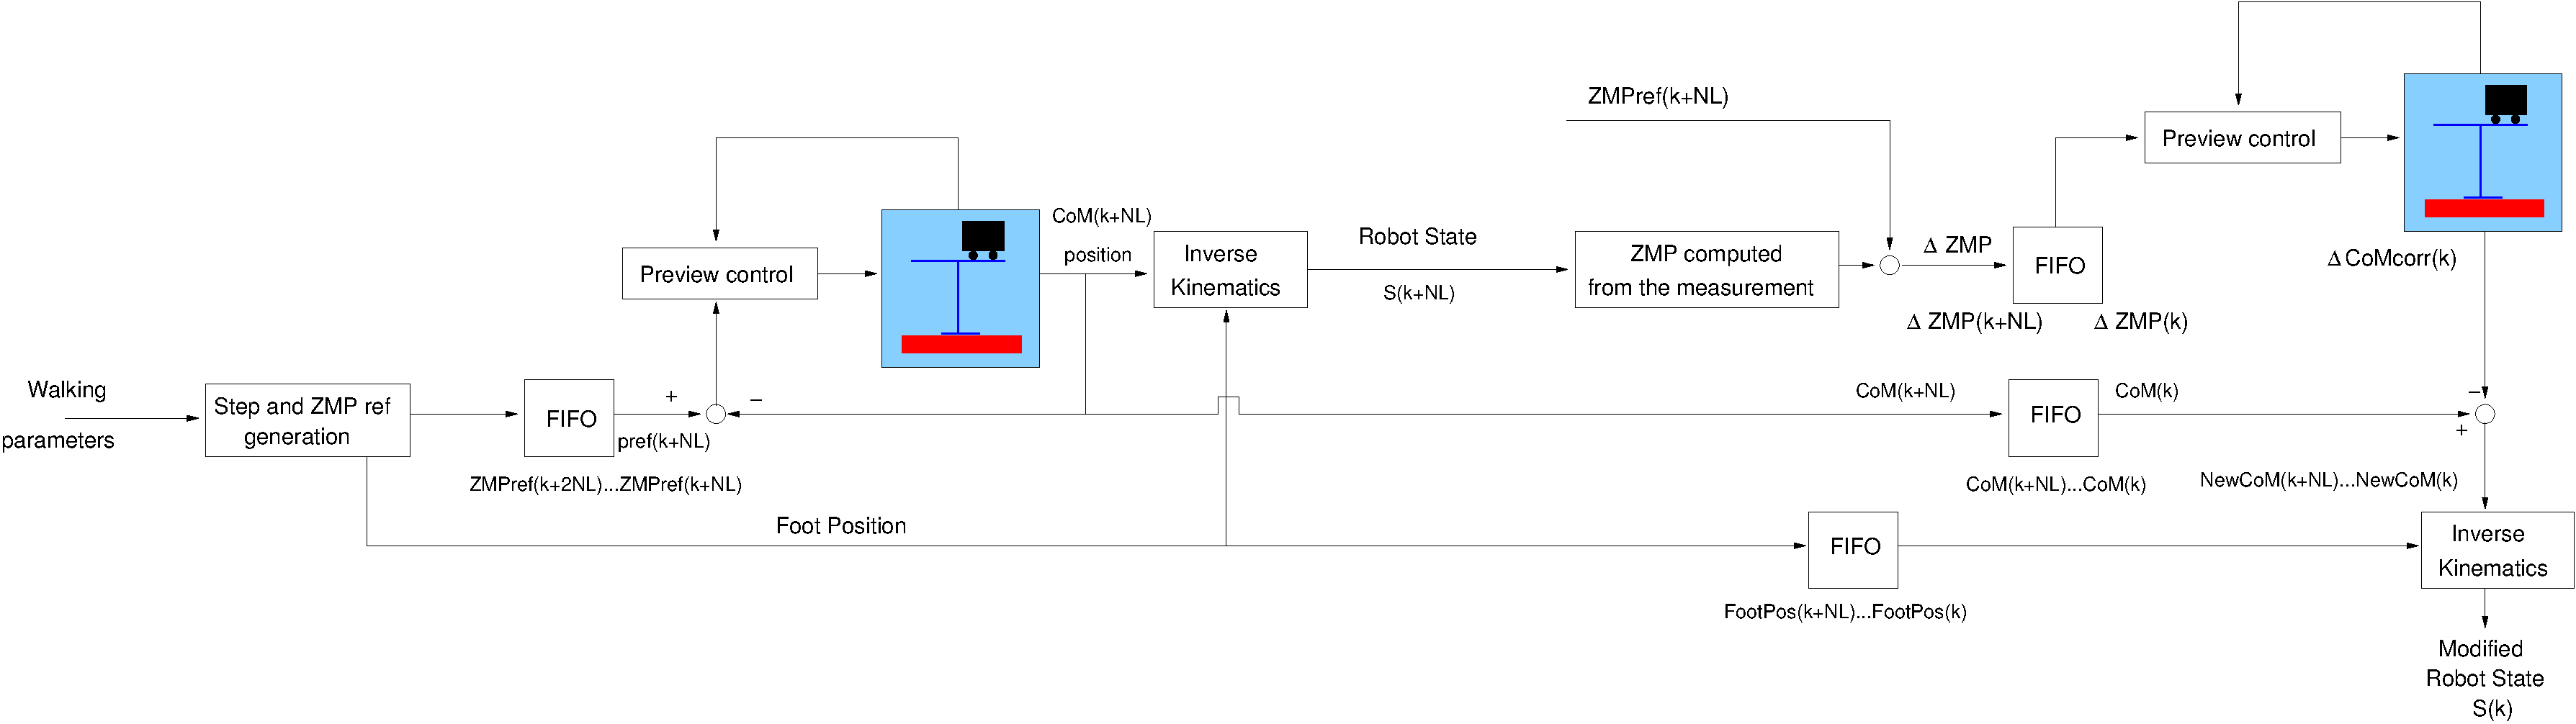
\includegraphics[angle=270,width=0.5\linewidth]{./figures/PatternGenerator/ZMPScheme2}
\caption{ZMP preview control taking into account the ZMP multibody }
\label{pic:ZMPScheme2}
\end{center}
\end{figure}
\clearpage
%
\clearpage
\begin{figure}[htb]
\begin{center}
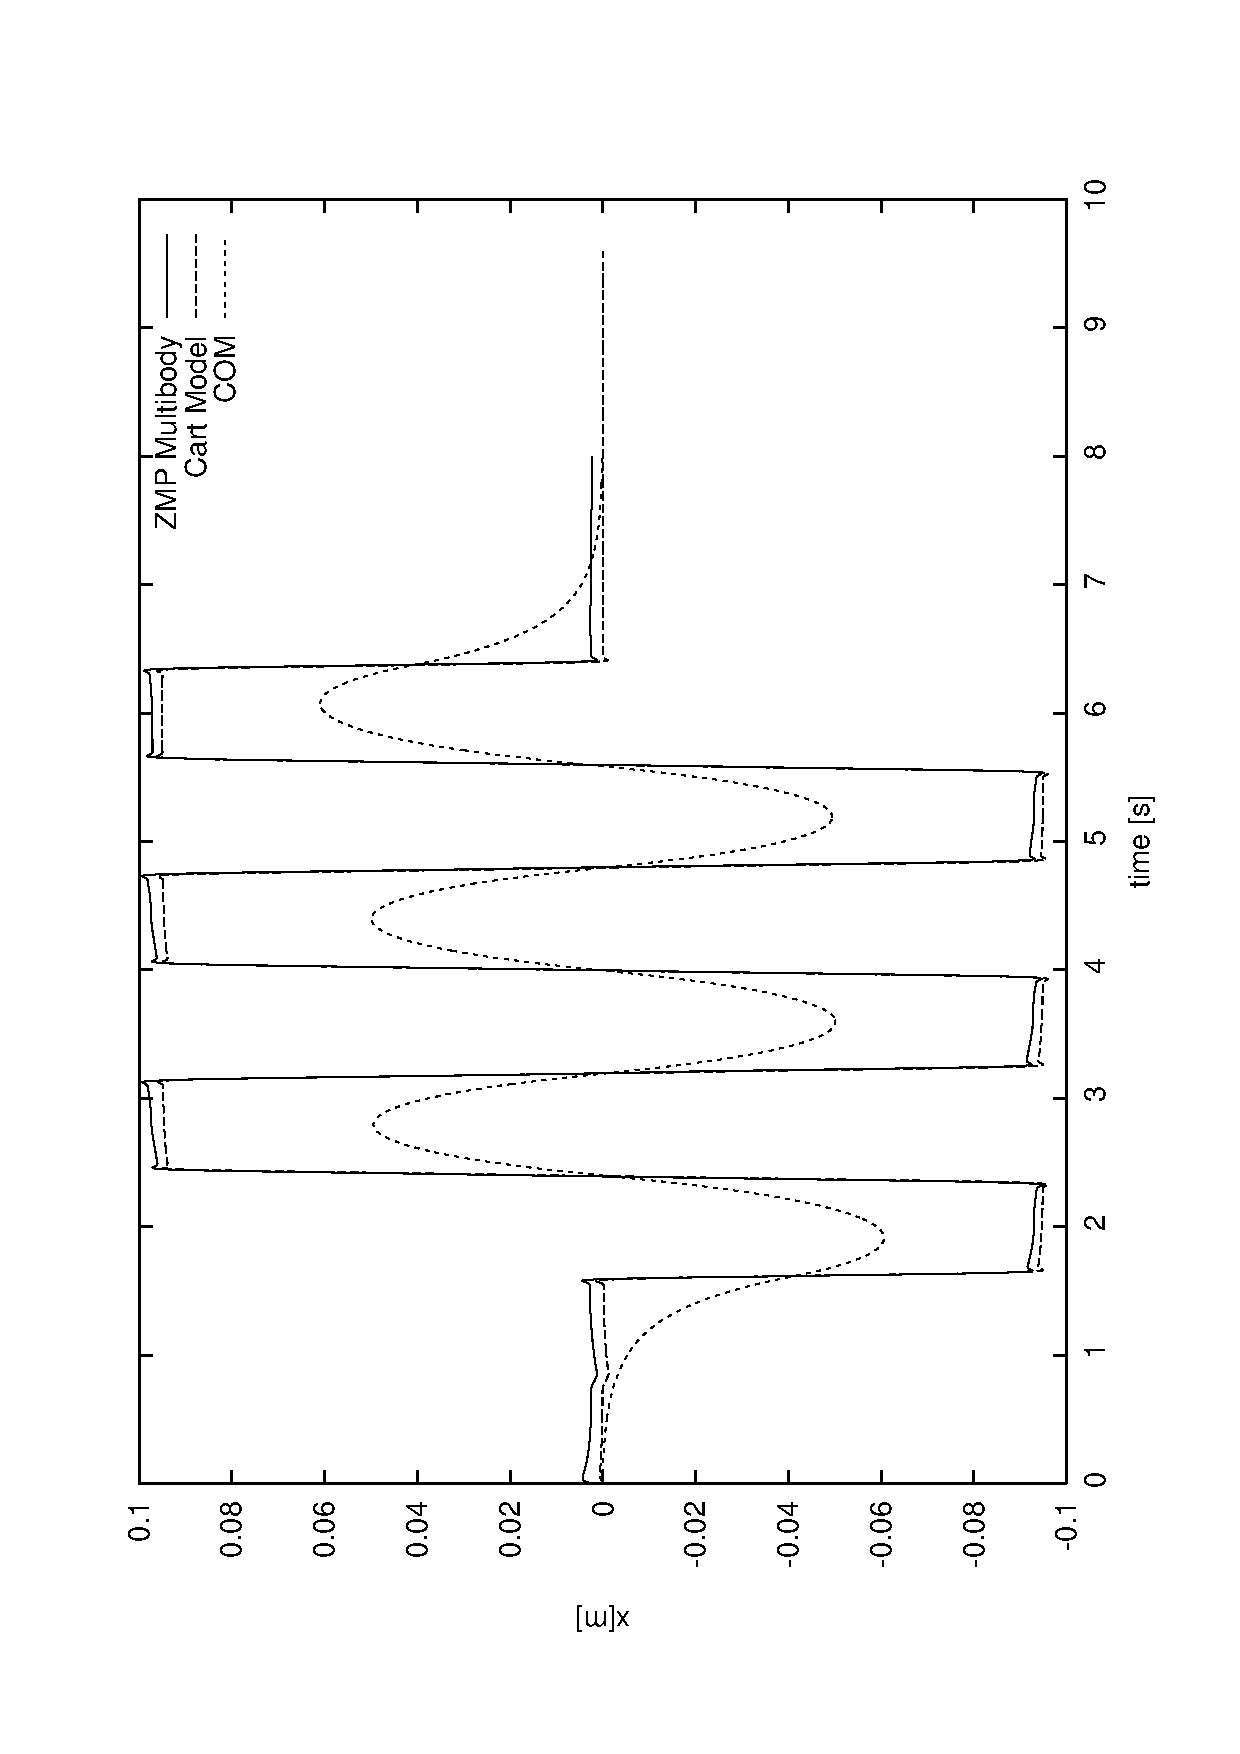
\includegraphics[width=\linewidth]{./figures/PatternGenerator/ThirdFigureZMPMB_X}
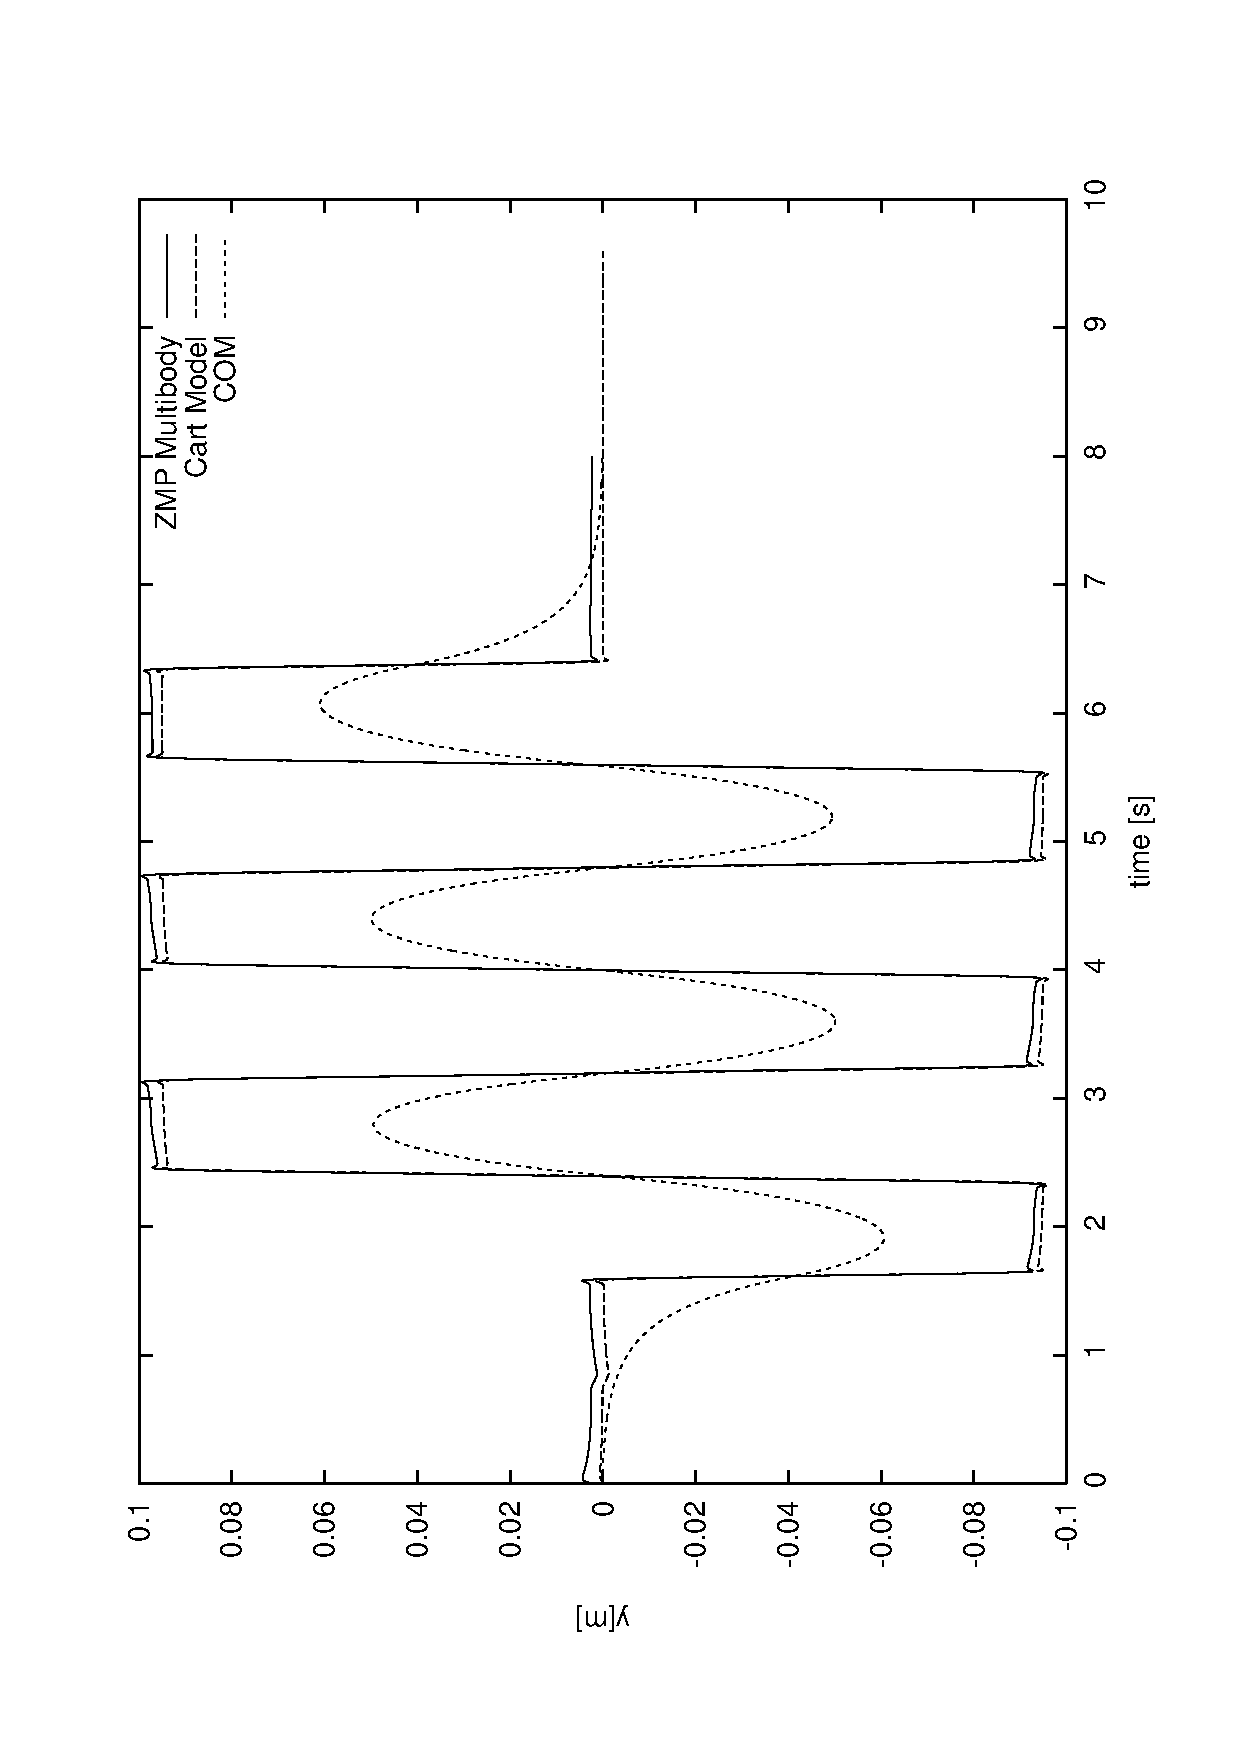
\includegraphics[width=\linewidth]{./figures/PatternGenerator/ThirdFigureZMPMB_Y}
\caption{Final ZMP after modification of the CoM}
\label{pic:ZMPMBcompensated}
\end{center}
\end{figure}
\clearpage

\subsection{References}
If you wish to generate new walking criterion, here are some reference curves.
\begin{figure}[htb]
\begin{center}
%\includegraphics[width=\linewidth]{./figures/PatternGenerator/LeftLegAngles}
\caption{Articular value for the right legs}
\label{pic:ZMPMBcompensated}
\end{center}
\end{figure}


\subsection{The angular momentum problem}
\begin{figure}[htb]
\begin{center}
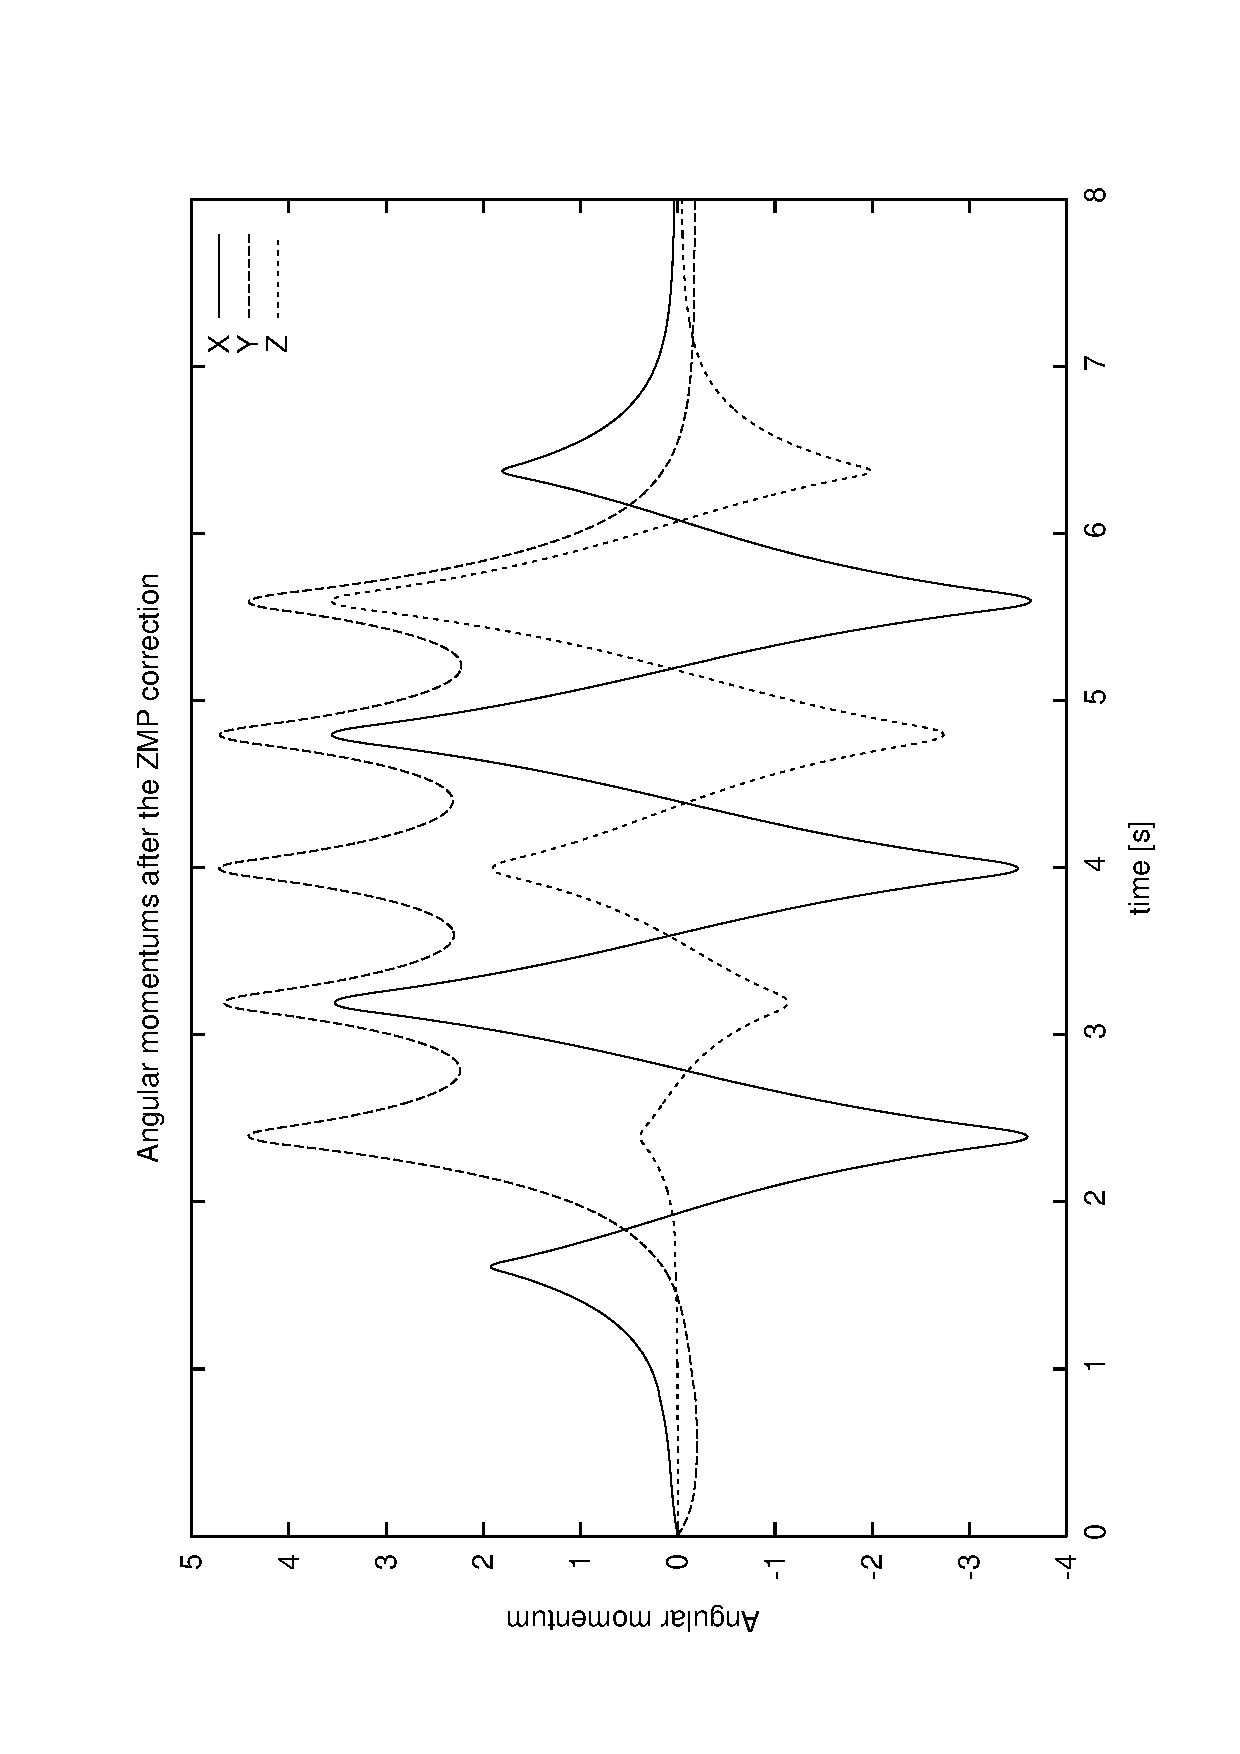
\includegraphics[width=\linewidth]{./figures/PatternGenerator/AngularMomentum}
\caption{Angular Momentum after ZMP correction}
\label{pic:AngularMomentum}
\end{center}
\end{figure}


The main problem related to this walking pattern is the generation of
unwelcome angular momentum around the z-axis. It creates strong rotation
for the robot during double-support phase. This is partly due to the fact that
in the previous part, the upper body motion has been totally ignored.
They are two possibilities to solve the problem: either design a heuristic 
aiming at compensate for the z-axis momentum, either implement a proper
control strategy to move the free upper-body's joints.
A heuristic involving only the arms is described, and the remaining part
of this document will described the concept of \textit{resolved momentum control}.

\subsection{Arm motion heuristic}

The main idea is to generate a motion with the arms which compensate the Z-axis moment 
by doing an arm movement. The basic idea is to generate a motion where the hand movement
has a linear relationship with the foot of the same side in the waist coordinates.

\section{Finding the weights for the preview control }

In this section we recall some well-known results in control theory in order to compute 
the gains for the ZMP preview control. Those notes are based on Kajita's book \cite{Kajita2005} p.147.

\subsection{The general scheme \cite{Katayama1985}}
The discrete system is	defined by three matrix A, b, c
     such as :
     \begin{equation}
	\begin{aligned}
     {\bf x}_{k+1} & =& {\bf A} {\bf x}_k + {\bf b} u_k \\
     p_k &=& {\bf cx}_k\\
	\end{aligned}
     \end{equation}

     The optimal critera considered here is :
     \begin{equation}
     J = \sum^{\infty}_{j=1} \{ Q(p^{ref}_j -p_j)^2 + Ru_j^2 \}
     \end{equation}

     where $ Q $ and $ R $ are also given as inputs.

    the solution is then 
     \begin{equation}
	\begin{aligned}	
     {\bf K} & \equiv  (R + {\bf b}^T{\bf Pb})^{-1}{\bf b}^T{\bf PA} \\
     f_i & \equiv  (R + {\bf b}^T{\bf Pb})^{-1}{\bf b}^T({\bf A}-{\bf bK})^{T*(i-1)}{\bf c}^TQ \\
	\end{aligned}
     \end{equation}


 where $ {\bf P} $ is solution of the following Riccati equation:
\begin{equation}
 {\bf P} = {\bf A}^T {\bf PA} + {\bf c}^TQ{\bf c} - {\bf A}^T{\bf Pb}(R + {\bf b}^T{\bf Pb})^{-1}{\bf b}^T{\bf PA}
\end{equation}

The computation of the solution can be done by using a software implementing the
method described in \cite{Arnold1984}. For this we used the publicly available
library called NetLib. In order to find ${\bf P}$, it is necessary to build
the Hamiltonian matrix:
\begin{equation}
{\bf H} = 
\left[
\begin{matrix}
{\bf A} & {\bf 0 } \\
-{\bf c}^TQ{\bf c} & {\bf I} \\
\end{matrix}
\right],
\;
{\bf E} = 
\left[
\begin{matrix}
{\bf I} & {\bf G } \\
{\bf 0} & {\bf A}^T \\
\end{matrix}
\right]
\end{equation}

with ${\bf G}= {\bf b} R^-1 {\bf b}^T$, and $I$ the identity matrix.
The function returns the left ${\bf V}$ and right ${\bf U}$ Schur vectors,
and ${\bf P}$ is such that :
\begin{equation}
{\bf P} = U_{21}U_{11}^{-1} 
\end{equation}

\subsection{Removing the offset of the ZMP}
	
The offset of the ZMP is directly dependant of the CoM's position.
Therefore in order to remove this problem, the derivated system is considered:
\begin{equation}
\begin{aligned}
     {\bf x}^*_{k+1} & =& \tilde{\bf A} {\bf x}_k + \tilde{{\bf b}} \Delta u_k \\
     p_k &=& \tilde{\bf c}{\bf x}^*_k\\
\end{aligned}
\end{equation}
with
\begin{equation}
\begin{aligned}
\Delta u_k & \equiv u_k - u_{k-1} \\
\Delta{\bf x}_k & \equiv {\bf x}_k - {\bf x}_{k-1}\\
 {\bf x}^*_k & \equiv 
	\left[ 
	\begin{matrix}
	p_k \\
	\Delta {\bf x}_k \\
	\end{matrix}
	\right] \\
\end{aligned}
\end{equation}



\subsection{Implementation of the weights computation}
     The resolution of the Riccati equation is taken from \cite{Laub1979}, and is
     based on a Schur form of the ${\bf P}$ matrix defined as:

     \begin{equation}
     {\bf Laub_Z} =
     \left(
     \begin{matrix}
     {\bf A} + {\bf GA}^{-T}{\bf c}^TQ{\bf c} & -{\bf GA}^{-T} \\
     -{\bf A}^{-T}{\bf c}^TQ{\bf c} & -{\bf A}^{-T} \\
     \end{matrix}
     \right)
     \end{equation}

\section{Momentum Equation}

The following are notes from Kajita et al \cite{Kajita2003b}.
\subsection{Momentum and joint velocities}
We represent a humanoid robot as a mechanism of tree structure whose root
is a free-flying base link (pelvis), a rigid body having 6 D.O.F. in 
3D space. We define the trame $\Sigma_B$ embedded in the base link whose translational
velocity and angular velocity are $\textit{\bf v}_b$ and $\textit{\bf w}_b$,
respectively. In addition, we define a $n \times 1$ column vector $\dot{\bf \theta}$
which contains velocities of all joints as its elements where $n$ is the total 
number of joints. The linear momentum $\textbf{P}$ ($3 \times 1$) and the
angular momentum ($4 \times 1$) of the whole mechanism are given by:
\begin{equation}
\left[
\begin{aligned}
\textbf{P}\\
\textbf{L}\\
\end{aligned}
\right] = 
\left[
\begin{matrix}
\tilde{m}\; {\bf E} & -\tilde{m}\;\hat{\bf r}_{B \rightarrow \tilde{c}} & {\bf M} _{\dot{\theta}} \\
{\bf 0}            & \tilde{\bf I}                                &{\bf H}_{\dot{\theta}} \\
\end{matrix}
\right]
\left[
\begin{aligned}
\textit{\bf v}_B \\
\textit{\bf w}_B \\
\dot{\bf \theta} \\
\end{aligned}
\right]
\label{eq:GlobalMomentum}
\end{equation}

where $\tilde{m}$ is the total mass of the robot, ${\bf E}$ is an identity matrix of size $3 \times 3$,
$\textbf{r}_{B \rightarrow \tilde{c}}$ is the $3 \times 1$ vector from the base link to the 
total center of mass (CoM) and ${\bf \tilde{I}}$ is the $3 \times 3$ inertia matrix with respect
to the CoM. ${\bf M}_{\dot{theta}}$ and ${\bf H}_{\dot{\theta}}$ are the $3 \times n$ inertia
matrices which indicate how the joint speeds affect to the linear momentum and the angular
momentum respectively. \^ is an operator which translates a vector of $3 \times 1$  into
a skew symmetric $3 \times 3$ matrix which is equivalent to a cross product.
\par
In this paper, we assume all vectors of position, velocity and angular velocity 
are represented in the Cartesian frame $\Sigma_O$ fixed on the ground.

\subsection{Constraints of foot contact}
Equation \ref{eq:GlobalMomentum} gives the total momentum of a flying robot.
However, when the robot is in contact with the ground we must take into account of constraints
that reduce the total D.O.F. of the system. 
The foot velocities $({\bf v}_{F_i}, {\bf w}_{F_i}$ of the frame $\Sigma_{F_i} \; (i=1,2)$ are
given by
\begin{equation}
\left[
\begin{aligned}
{\bf v}_{F_i} \\
{\bf w}_{F_i}\\
\end{aligned}
\right]
=
\left[
\begin{matrix}
{\bf E} & \hat{\bf r}_{B \rightarrow F_i} \\
{\bf 0} & {\bf E}\\
\end{matrix}
\right]
\left[
\begin{aligned}
{\bf v}_{B} \\
{\bf w}_{B}\\
\end{aligned}
\right]
+
{\bf J}_{leg_i} \dot{\bf \theta}_{leg_i}
\end{equation}
where ${\bf J}_{leg_i}$ is a Jacobian matrix ($ 6 \times 6$ ) calculated from the leg configuration,
${\bf r}_{B \rightarrow F_i}$ is a position vector $(3 \times 1 )$ from the base frame to the foot
frame and $\dot{\bf \theta}_{leg_i}$ is the joint speed vector ($ 6 \times 1 $) of each leg.
If ${\bf J}_{leg_i} \; (i=1,2)$  are non singular, the vectors for the leg are given by:

\begin{equation}
\dot{\bf \theta}_{leg_i} = {\bf J}^{-1}_{leg_i}
\left[
\begin{aligned}
{\bf v}_{F_i} \\
{\bf w}_{F_i} \\
\end{aligned}
\right]
- 
{\bf J}^{-1}_{leg_i}
\left[
\begin{matrix}
{\bf E} & \hat{\bf r}_{B \rightarrow F_i} \\
{\bf 0} & {\bf E}\\
\end{matrix}
\right]
\left[
\begin{aligned}
{\bf v}_{B} \\
{\bf w}_{B} \\
\end{aligned}
\right]
\label{eq:ThetaLeg}
\end{equation}
Let us divied the whole joint speed vector into the leg parts and the free part as:
\begin{equation}
\dot{\bf \theta} = [ \dot{\bf \theta}^T_{leg_1} \dot{\bf \theta}^T_{leg_2} 
  \dot{\bf \theta}^T_{free} ]^T
\end{equation}
where $\dot{\bf \theta}_{free}$ is the joint speed for waist, arms and head.
We also divide the corresponding inertia matrices as:
\begin{equation}
\begin{aligned}
{\bf M}_{\dot{\theta}} &= [ {\bf M}_{leg_1} \; {\bf M}_{leg_2} \; {\bf M}_{free} ], \\
{\bf H}_{\dot{\theta}} &= [ {\bf H}_{leg_1} \; {\bf H}_{leg_2} \; {\bf H}_{free} ]. \\
\end{aligned}
\end{equation}
Then we can rewrite the momentum equations \ref{eq:GlobalMomentum} as:
\begin{equation}
\left[
\begin{aligned}
\textbf{P}\\
\textbf{L}\\
\end{aligned}
\right] = 
\left[
\begin{aligned}
\tilde{m}\; {\bf E} & -\tilde{m}\; \hat{\bf r}_{B \rightarrow \tilde{c}}  \\
{\bf 0}           &  \tilde{\bf I}                                 \\
\end{aligned}
\right]
\left[
\begin{aligned}
\textit{\bf v}_B \\
\textit{\bf w}_B \\
\end{aligned}
\right]
+
\sum^{2}_{i=1}
\left[
\begin{aligned}
{\bf M} _{leg_i}\\
{\bf H} _{leg_i}\\
\end{aligned}
\right]
\dot{\bf \theta}_{leg_i} 
+
\left[
\begin{aligned}
{\bf M} _{free}\\
{\bf H} _{free}\\
\end{aligned}
\right]
\dot{\bf \theta}_{free} 
\label{eq:SplittedGlobalMomentum}
\end{equation}
By substituing \ref{eq:ThetaLeg} into \ref{eq:SplittedGlobalMomentum},
we obtain the momentum equation under the constraint as:
\begin{equation}
\left[
\begin{aligned}
\textbf{P}\\
\textbf{L}\\
\end{aligned}
\right] = 
\left[
\begin{matrix}
{\bf M}^*_{B} & {\bf M}_{free}\\
{\bf H}^*_{B} & {\bf H}_{free}\\
\end{matrix}
\right]
\left[
\begin{matrix}
{\bf \xi}_{B}\\
\dot{\theta}_{free}\\
\end{matrix}
\right]
+
\sum_{n=1}^{2}
\left[
\begin{matrix}
{\bf M}^*_{F_i}\\
{\bf H}^*_{F_i}\\
\end{matrix}
\right]
\dot{{\bf \xi}}_{F_i},
\label{eq:ConstraintedMomentum}
\end{equation}
where
\begin{equation*}
\begin{aligned}
{\bf \xi}_B & \equiv [ {\bf v}^T_{B}\; {\bf w}^T_B]^T\\
{\bf \xi}_{F_i}& \equiv [ {\bf v}^T_{F_i}\; {\bf w}^T_{F_i}]^T\\
\left[
\begin{matrix}
{\bf M}^*_{B}\\
{\bf H}^*_{B}\\
\end{matrix}
\right] &
\equiv
\left[
\begin{matrix}
\tilde{m}\; {\bf E} & -\tilde{m}\; \hat{\bf r}_{B \rightarrow \tilde{c}} \\
{\bf 0}           & - \tilde{\bf I}                                 \\
\end{matrix}
\right]
- \sum^{2}_{n=1} 
\left[
\begin{matrix}
{\bf M}^*_{F_i}\\
{\bf H}^*_{F_i}\\
\end{matrix}
\right]
\left[
\begin{matrix}
\tilde{m}\; {\bf E} & -\tilde{m}\; \hat{\bf r}_{B \rightarrow F_i} \\
{\bf 0}           & {\bf E}                                 \\
\end{matrix}
\right], \\
\left[
\begin{matrix}
{\bf M}^*_{F_i}\\
{\bf H}^*_{F_i}\\
\end{matrix}
\right]
& \equiv
\left[
\begin{matrix}
{\bf M}_{leg_i}\\
{\bf H}_{leg_i}\\
\end{matrix}
\right]
{\bf J}^{-1}_{leg_i}.
\end{aligned}\\
\end{equation*}
The second term in the right hand side of \ref{eq:ConstraintedMomentum} indicates
the extra momentum generated by specifying the foot speed.


	
\section{Resolved Momentum Control}

\subsection{Setting momentum reference}

For every mechnical system, no matter how its structure or behavior is complicated,
we can determine the position of the CoM $\tilde{\bf c}$,
the linear momentum ${\bf P}$ and the angular momentum ${\bf L}$
for the total mechanism.
\par
Dividing the total linear momentum ${\bf P}$  by the total mass $\tilde{m}$,
we obtain the translational speed of the CoM:
\begin{equation}
\frac{d}{dt}\tilde{\bf c} = \frac{\bf P}{\tilde{m}}
\end{equation}
Thus, we can control the position of the CoM by manpulating the linear momentum.
\par
As the extension of this, we propose a method of control or pattern generation
by manipulating the total (linear and angular) momentum. Let us call this
method the \textit{Resolved Momentum Control}. The reference motion of a humanoid robot
 can be specified by assuming a rigid body whose mass and moment of inertia
are equal to the target. However, we cannot associate the orientation of this 
imaginary object to the robot, since a rigid body can not hold enough information
to represent the internal structure of the multi-body system.

\subsection{Momentum selection and control by pseudo-inverse}
In many applications, we do not have to specify all six elements of the momentum.
Moreover, in some case we encounters a numerical unstability by specifying the all
elements of the reference momentum.
Therefore we introduce a selection matrix ${\bf S}$ which is $l\times 6 (0 \le l \leq 6 $)
to pick up the elements of the momentum to be controlled. The selection of the momentum
is given by 
\begin{equation}
{\bf S} \equiv 
\left[
\begin{matrix}
{\bf e}^T_{s_1} \\
. \\
. \\
.\\
{\bf e}^T_{s_l} \\
\end{matrix}
\right],
\end{equation}
where ${\bf e}_{s_i}$ is a column vector of $6 \times 1$ that has one at $s_i$-th row 
and zeros for the rest. $s_i$ specifies the element of the momentum we want to pick up.
Transposing the second term of \ref{eq:SplittedGlobalMomentum} from the right side to 
the left side, then multiplying ${\bf S}$ from left, we obtain the following equation:
\begin{equation}
{\bf y} = {\bf A} 
\left[
\begin{matrix}
\xi_{B}\\
\dot{\theta}_{free}\\
\end{matrix}
\right]
\label{eq:TheLinearSystem}
\end{equation}
where
\begin{equation}
{\bf y} = {\bf S}
\left\{
\begin{matrix}
\left[
\begin{matrix}
{\bf P}^{ref} \\
{\bf L}^{ref} \\
\end{matrix}
\right]
-
\sum^{2}_{n=1}
\left[
\begin{matrix}
{\bf M}^*_{F_i} \\
{\bf H}^*_{F_i} \\
\end{matrix}
\right]
\xi^{ref}_{F_i}
\end{matrix}
\right\}
\end{equation},
\begin{equation}
{\bf A} \equiv {\bf S}
\left[
\begin{matrix}
{\bf M}^*_B & {\bf M}_{free}\\
{\bf H}^*_B & {\bf H}_{free}\\
\end{matrix}
\right]
\end{equation}
Here ${\bf P}^{ref}$ is the reference linear momentum,
${\bf L}^{ref}$ is the reference angular momentum and
$\xi^{ref}_{F_i}$ is the reference velocity for each foot.
\par
Using \ref{eq:TheLinearSystem}, the target speed which realizes the
reference momentum and the speed ($\xi^{ref}_B, \dot{\theta}^{ref}$)
is calculated as the least square solution by:
\begin{equation}
\left[
\begin{matrix}
\xi_B \\
\dot{\bf \theta}_{free}
\end{matrix}
\right]
=
{\bf A}^{\dagger}{\bf y}
+ ({\bf E} - {\bf A}^{\dagger}{\bf A})
\left[
\begin{matrix}
\xi_B^{ref} \\
\dot{\bf \theta}_{free}^{ref}\\
\end{matrix}
\right]
\end{equation},
where ${\bf A}^{\dagger}$ is a pseudo-inverse (the least-squares inverse) of
${\bf A}$. This equation gives the Resolved Momentum Control.


\subsection{Calculation of the interia matrices}
In this section we describe a method to calculate the inertia matrices
${\bf M}_{\dot{\theta}}$ and ${\bf H}_{\dot{\theta}}$, which appears
in \ref{eq:GlobalMomentum}.
\par
Figure 
%\ref{}
shows a part of the robot links containing the joint $j-1$ and joint $j$.
We assume that the robot can rotate its joints with specified speed inder the 
proper control law like PD feedback. The joint $j$'s rotation with speed
$\dot{\theta}_j$ yields additional linear and angular momentum. of

\begin{equation}
\begin{aligned}
{\bf P}_j &= {\bf w} \times ( \tilde{\bf c}_j - {\bf r}_j ) \tilde{m}_j \\
\end{aligned}
\label{eq:IterativeLinearMomentum}
\end{equation}

\begin{equation}
\begin{aligned}
{\bf L}_j &= \tilde{\bf c}_j \times {\bf P}_j + \tilde{\bf I}{\bf w}_j \\
\end{aligned}
\label{eq:IterativeAngularMomentum}
\end{equation}
\begin{equation}
\begin{aligned}
{\bf w}_j &= {\bf a}\dot{\theta}_j \\
\end{aligned}
\label{eq:IterativeAngularSpeed}
\end{equation}

where ${\bf r}_j$ and ${\bf a}_j$ are the position vector and the rotation axis vector
of the joint $j$, $\tilde{m}_j$, $\tilde{c}_j$ and $\tilde{\bf I}_j$ mean mass,
center of mass and inertia tensor of all link structure driven by the joint $j$.
\par
Now, the columns of the inertia matrices corrspondig to the joint $j$ are determined
by the following equations:
\begin{equation}
\begin{aligned}
{\bf m}_j & \equiv {\bf P}/\dot{\theta}_j, \\
\end{aligned}
\label{eq:JointLinearMomemtum}
\end{equation}
\begin{equation}
\begin{aligned}
{\bf h}_j & \equiv {\bf L}/\dot{\theta}_j, \\
\end{aligned}
\label{eq:JointAngularMomentum}
\end{equation}
where ${\bf m}_j$  and ${\bf h}_j$ are $3 \times 1$ vectors. By comparing 
\ref{eq:IterativeLinearMomentum} and \ref{eq:JointLinearMomemtum}, we obtain
${\bf m}_j$. Likewise, by comparing \ref{eq:IterativeAngularSpeed}
and \ref{eq:JointAngularMomentum} we obtain ${\bf h}_j$ by:
\begin{equation}
{\bf m}_j = {\bf a}_j \times ( \tilde{\bf c}_j - {\bf r}_j) \tilde{m}_j
\label{eq:IterativeLinearMomentum2}
\end{equation}
\begin{equation}
{\bf h}_j = \tilde{\bf c}_j \times ( \tilde{\bf m}_j ) + \tilde{\bf I}_j a_j
\label{eq:IterativeLinearMomentum2}
\end{equation}

Using these column vectors, the inertia matrices ${\bf M}_{\dot{\theta}}$ and 
${\bf H}_{\dot{\theta}}$ are constructed like :
\begin{equation}
{\bf M} =  [ {\bf m}_1, {\bf m}_2, ... {\bf m}_n] \\
\end{equation}
\begin{equation}
{\bf H}_{\dot{\theta}} = ^{0}{\bf H}_{\dot{\theta}} - \hat{\tilde{\bf c}} {\bf M}_{\dot{\theta}} \\
\label{eq:ConvertionOfAngularMomentumIntoRobotCoMFrame}
\end{equation}
\begin{equation}
^{0}{\bf H}_{\dot{\theta}} =  [ {\bf h}_1, {\bf h}_2, ... {\bf h}_n] \\
\end{equation}

Equation \ref{eq:ConvertionOfAngularMomentumIntoRobotCoMFrame} converts the angular 
momentum from the ground frame into the angular momentum in the robot's CoM frame.
\par
We can calculate $\tilde{m}_j$,$\tilde{\bf c}_j$ and $\tilde{\bf I}_j$ from an 
extremity to the body side by using a recurisve algorithm. Assuming we have 
already calculated $\tilde{m}_j, \tilde{\bf c}_j$ and $\tilde{\bf I}_j$ about joint $j$,
the parameters of adjacent point $j$-1  can be calculated as:
\begin{equation}
\begin{aligned}
\tilde{m}_{j-1} & = \tilde{m}_j + \tilde{m}_{j-1}\\
\tilde{\bf c}_{j-1} & = ( \tilde{m}_j\tilde{\bf c}_j + m_{j-1}{\bf c}_{j-1})/(\tilde{m}_j + m_{j-1}) \\
\tilde{\bf I}_{j-1} &= \tilde{\bf I}_j + \tilde{m}_j D (\tilde{\bf c}_j - \tilde{\bf c}_{j-1})
		+ {\bf R}_{j-1}{\bf I}_{j-1} {\bf R}^T_{j-1} 
	+ m_{j-1} D ({\bf c}_{j-1} - \tilde{\bf c}_{j-1})\\
\tilde D(r) & \equiv \hat{\bf r}\tilde{\bf r}\\
\end{aligned}	
\end{equation}

where ${\bf R}_{j-1}$, $m_{j-1}$ and ${\bf I}_{j-1}$ are $3 \times 3$ orientation matrix, mass
and inertia tensor around the center of the $j-1$th link respectively.


\subsection{Walking using the Resolved Momentum Control}
In this section we evaluate the motion generated by the Resolved Momentum Control 
using the HRP-2 humanoid robot to realize a walking motion.
The target momentum control is given such that the robot's CoM follows
given references by

\begin{equation}
P^{ref}_{x,y} = \tilde{m}K_p (\tilde{c}_{x,y}^{ref} - \tilde{c}_{x,y} )+ \dot{\tilde{c}}^{ref}_{x,y}
\label{eq:XYLinearMomentum}
\end{equation}
\begin{equation}
P^{ref}_{z} = \tilde{m} K_p (z_B^{ref} - z_B)
\label{eq:ZLinearMomentum}
\end{equation}
\begin{equation}
{\bf L}^{ref} = {\bf 0}_{3 \times 1}
\end{equation}

where $K_p$ is a feedback gain which compensates the error caused by time derivative of Jacobian,
$\tilde{\bf c}^{ref}$ is the target position of CoM, $\dot{\tilde{\bf c}}^{ref}$ is the target
speed of CoM and $z_B$ is the target height of the pelvis. As specified by $\cite{}$
we made special treatment for the $z$ element of the linear momentum. This is because the constant
pelvis height is desirable for most of the case.
\par
The references for the right and left foot ${\bf \xi}^{ref}_{F_1}$ and ${\bf \xi}^{ref}_{F_2}$
are computed according to the method described previously.


\section{To change the library}

\begin{figure}[htb]
\begin{center}
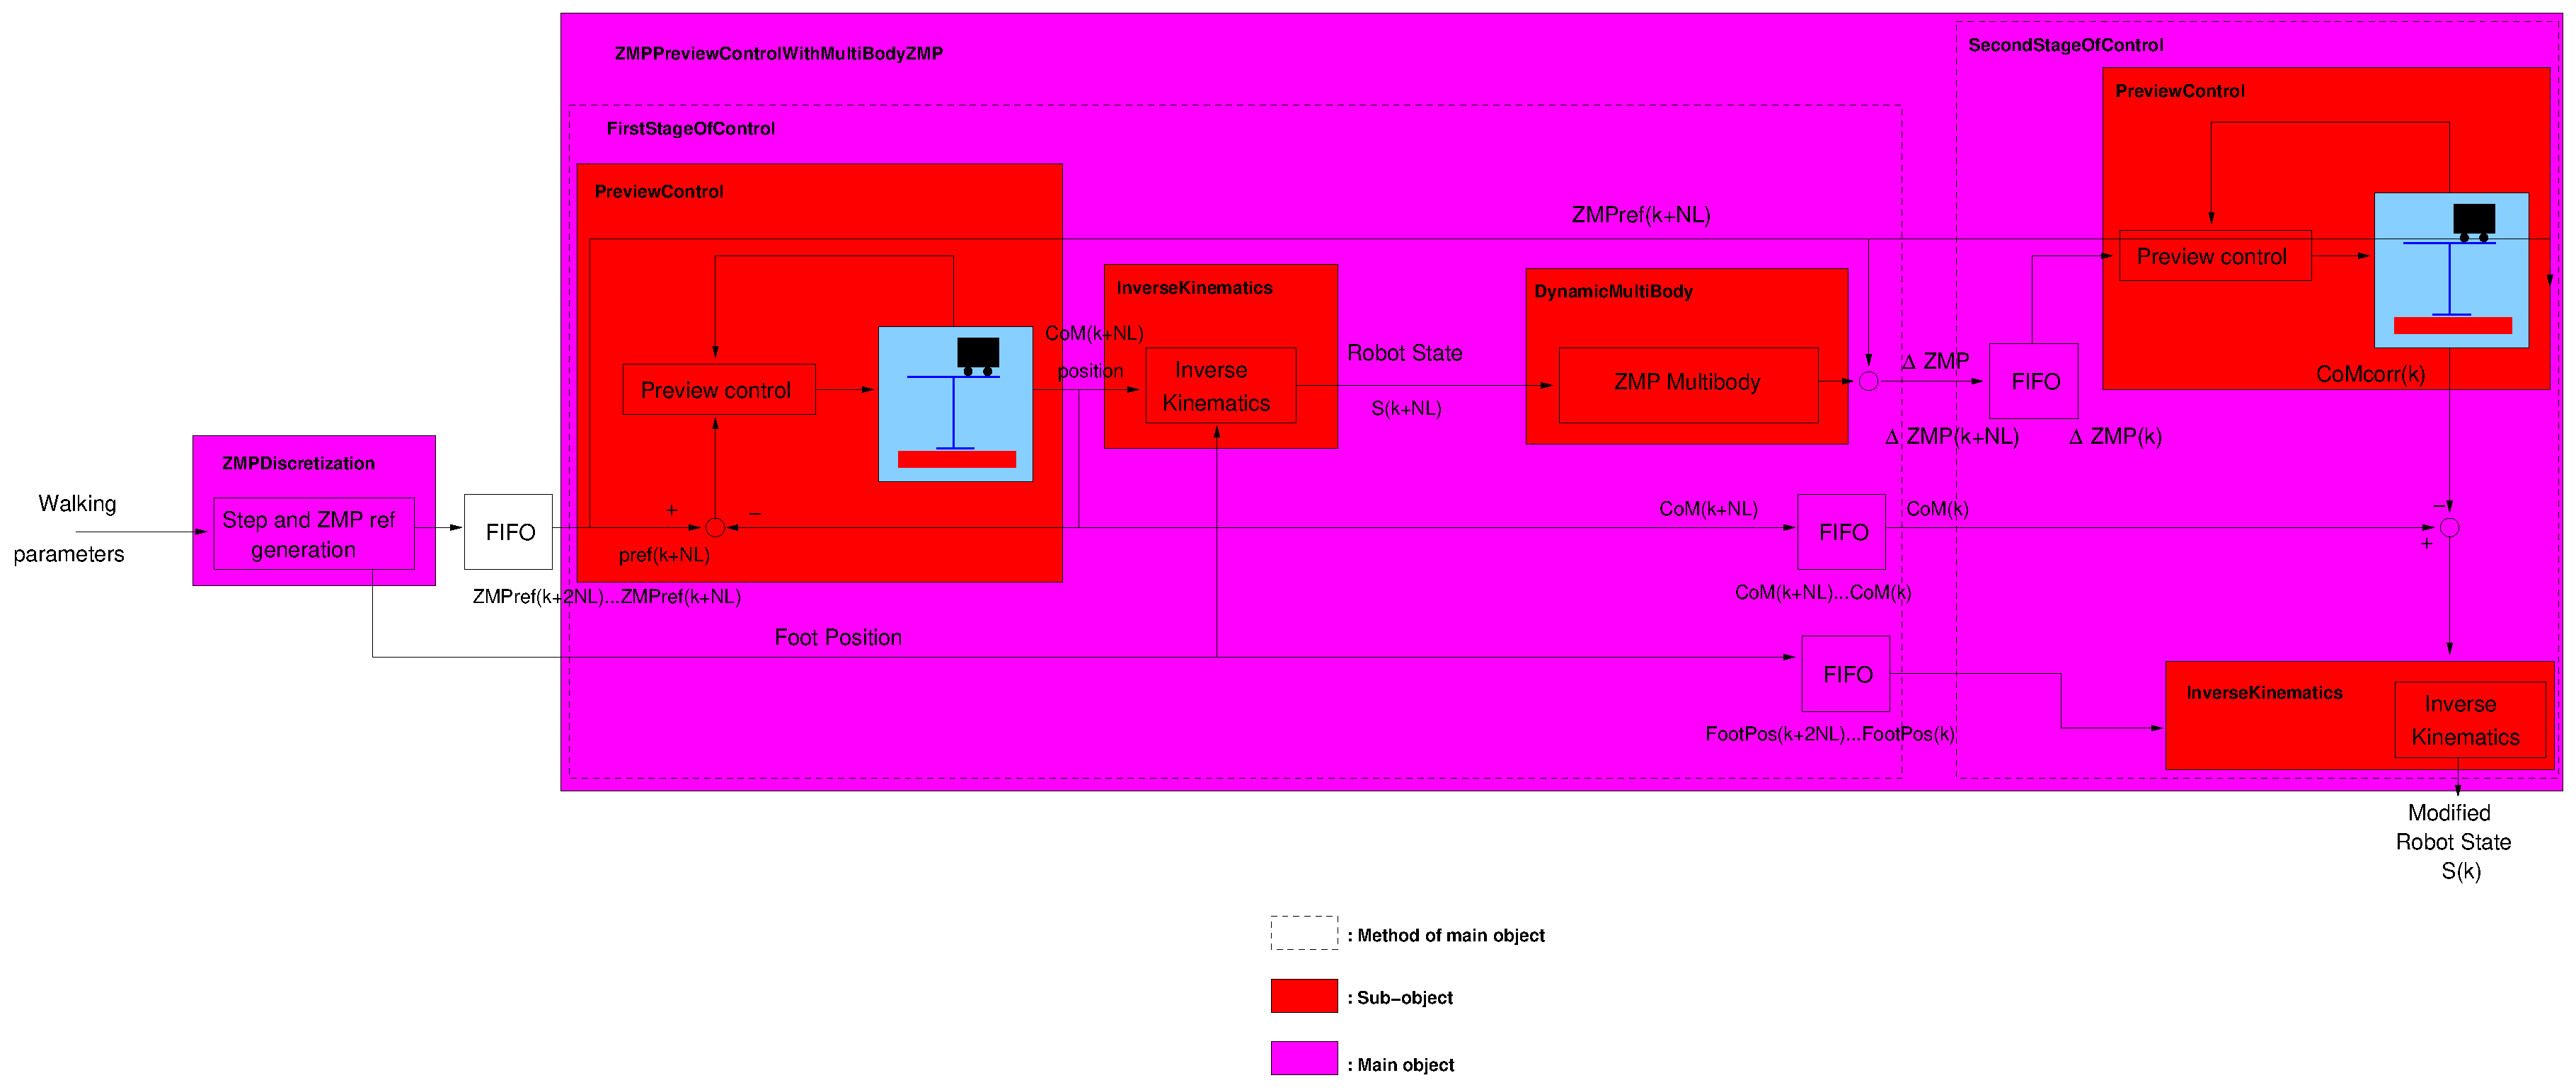
\includegraphics[angle=270,width=0.7\linewidth]{./figures/PatternGenerator/ZMPSchemeSoftware}
\caption{Overall structure of the library based on the control scheme.}
\label{pic:OverallStructure}
\end{center}
\end{figure}

\subsection{Introduction}
The overall architecture of the library relies on the ZMP preview control scheme as explained previously.
The main objects are depicted in Fig. \ref{pic:OverallStructure} and are :
\begin{itemize}
\item {\bf ZMPDiscretization}: Transform the stack of foot position in ZMP and position trajectories to be used
every 5 ms.
\item {\bf ZMPPreviewControlWithMultiBodyZMP}: Realize the control of the ZMP trajectory using Preview Control, and 
an estimation of the robot's multibody ZMP. The object is made of two main methods {\bf FirstStageOfControl} and {\bf SecondStageOfControl}.
The sub-objects used are:
\begin{itemize}
\item {\bf PreviewControl}: Object which implements the preview control of the cart-table model.
\item {\bf InverseKinematics}: Object which implements the simplified inverse kinematics for the legs and the arms.
\item {\bf DynamicMultibody}: Computes the dynamic of the robot to get the multibody's ZMP.
\end{itemize}
\end{itemize}

\subsection{ZMPDiscretization}
This object transforms a stack of support foot position into a stack of ZMP, orientation and foot position every 5 ms.
The position in X and Y follow third orders polynomial for the foot and the ZMP position. 
\par
This object is currently assume to produce a full motion from the beginning where the robot is at the half-sitting position 
up to the end where the robot is also at the half-sitting position.
The method in charge of this is {\bf GetZMPDiscretization}. This function should be
changed in order to have a dynamical planning of the foot.
The motion is splitted into three parts:
\begin{enumerate}
\item The beginning of the motion which adds the time of the preview control window to slowly prepare
the robot to move towards the first support foot.
\item For each step there is a decomposition of three phases: 
\begin{enumerate}
\item a half-double phase for the non-support foot take-off, 
\item a flying phase,
\item a landing phase. 
\end{enumerate}
\item A final phase where the ZMP is the middle of the two last position of the support foot.
\end{enumerate}
\par
The polynomials used for the foot generation can be changed, but happen to be a problem for stability. 
Indeed the acceleration is set to be zero at the beginning 
and at the end of the trajectory with a fifth order polynomial. For the foot this prevent compensation for the momentum around 
the Z-axis.

{\bf TODO}: They are unuseful code inside this part which should be removed.
The hand behavior should be put here. The code should more versatile for dynamic planning.

\subsection{Preview Control}
This object implements the preview control described previously. 
It is assumed that the control parameters and the size of the window would be provided through
a parameters file. The current format is as follows:
\begin{verbatim}
ZMP_Height
Sampling_Period
Preview_Control_Time
Kx_0 Kx_1 Kx_2
Ks
F_0 F_1 ... F_SizeOfPreviewWindow
\end{verbatim}
where $SizeOfPreviewWindow = Preview\_Control\_Time \times Sampling\_Period$.
\par
{\bf TODO:} VNL offers the capabilities to solve the Ricatti equations 
associated with the linear system. The Schur decomposition could be used for that.

\subsection{Dynamic Multi Body}
This object reads a VRML file following the format of OpenHRP2 and creates a tree
of bodies. Using the {\bf ForwardVelocity} method it is possible to simulate the
dynamic of the robot by specifying the position, orientation and linear velocity
of a root body. This root body is set by default to the waist when reading the
object at start. It can be modified using {\bf SpecifyTheRootLabel}. 
To make it work, the joint position and their speed must be also provided.
\par
The computation of ZMP is done by keeping track of the linear and angular momentum
through {\bf GetPandL}. You have to perform a simple difference for both of them between two iterations
and call {\bf CalculateZMP} which takes them as an input.
DynamicMultiBody has been modified to compute the matrices needed for the resolved momentum control.
See TestFootPrint2.cpp in src for a practical example.

{\bf TODO}: Add the angular velocity for the {\bf ForwardVelocity} method.
Remove the french naming.

\subsection{ZMPPreviewControlWithZMPMultiBody}

This object implements the queues and the synchronization between the different object
for controlling one iteration of the overall scheme. Once the ZMP stack has been build,
only one position for each foot and for the ZMP must be provided.
The delays between the queues have to be carefully chosen after the explanation provided previously.
The corresponding joint values are then computed and are provided as well as the CoM
position and orientation.
This object should not be modified unless the preview control window is itself modified.

\chapter{The Upper body Motion}

\section{Walking Mode inside the Pattern Generator V.2 }

\begin{table}
\begin{tabular}{|c|c|} \hline
Walk Mode & Meaning \\ \hline \hline
{\bf 0} & Normal walking \\
{\bf 1} & Modification of the hip height \\
{\bf 2} & Stepping over \\
{\bf 3} & Planification of the upper body motion with way-points \\
{\bf 4} & Let the other plugin modify the upper body \\ \hline 
\end{tabular}
\caption{Handling of the upper body motion according to the walking mode}
\end{table}
